%%%%%%%%%%%%%%%%%%%%%%%%%%%%%%%%%%%%%%%%%%%%%%%%%%%%%%%%%%%%%%%%%
\section{Aerodynamics and Aircraft Performance}
%%%%%%%%%%%%%%%%%%%%%%%%%%%%%%%%%%%%%%%%%%%%%%%%%%%%%%%%%%%%%%%%%
This section provides basic theoretical understanding about the aircraft performance analysis. Using this theory will allow us to evaluate basic requirements for engine design analysis, including thrust, take-off and landing, and cruise performance. To link basic thrust requirements to the engine performance, we will then derive the thrust equation and propeller theory to determine engine performance requirements. 

%%%%%%%%%%%%%%%%%%%%%%%%%%%%%%%%%%%%%%%%%%%%%%%%%%%%%%%%%%%%%%%%%
\subsection{Aerodynamics: Drag, Lift, and Airfoil Theory}
%%%%%%%%%%%%%%%%%%%%%%%%%%%%%%%%%%%%%%%%%%%%%%%%%%%%%%%%%%%%%%%%%
The aerodynamic analysis closely follows Secs. 5 and 6 of Anderson \cite{ANDERSON_INTRO_TO_FLIGHT_BOOK2012}. Here we consider an infinitely long airfoil. Forces acting on the airfoil, relevant to our analysis, include the lift and drag (see \cref{FIG_AIRFOIL}). 

%================================================================
\begin{figure}[!h!]
\begin{center}
  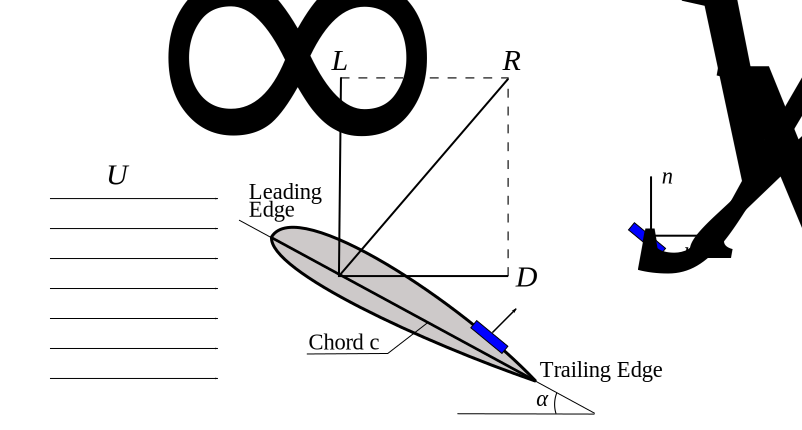
\includegraphics[scale =0.56]{airfoilDiagram}
  \caption{\label{FIG_AIRFOIL}Forces on an airfoil with $U_\infty$: free-stream velocity; $\alpha$ angle of attack; $L$ lift force; $D$ drag force; and $c$: chord.}
\end{center}
\end{figure}
%================================================================

The {\it lift force} is defined as the force on an airfoil acting in the perpendicular direction to flight path (neglecting viscous stress contributions):
\begin{equation}
  \begin{split}
    L =& - \oint p\nvec_y\cdot d \Avec\\
     =& \left.\int^c_0 p \nvec_y\cdot d \Avec\right|_\text{lower side} - \left.\int^c_0 p \nvec_y\cdot d \Avec\right|_\text{upper side} \, \text{.}
  \end{split}
\end{equation}
The {\it{lift coefficient}} is defined as
\begin{equation}
  C_L = \f{L}{q_\infty S} \, \text{,}
\end{equation}
where the dynamic pressure $q_\infty$ is defined as
\begin{equation}
   q_\infty = \f{1}{2}\rho_\infty U^2_\infty \, \text{.}
\end{equation}
Similarly, we can also define the {\it sectional lift coefficient}
\begin{equation}
  c_l = \f{l}{q_\infty c} \, \text{,}
\end{equation}
where $l$ is the lift per unit length, and $c$ is the chord.

%================================================================
\begin{figure}[!b!]
  \begin{center}
    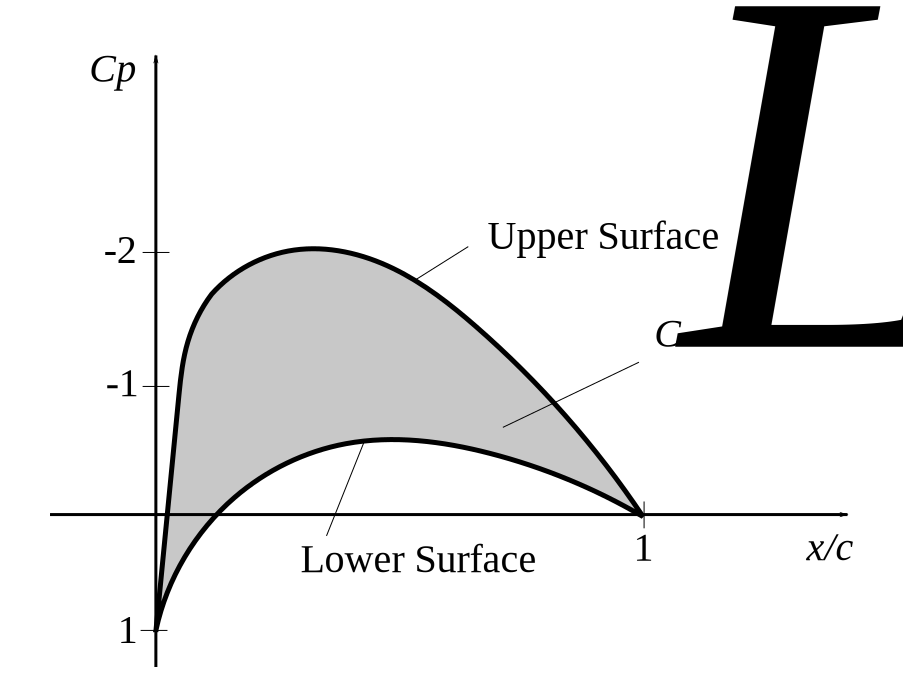
\includegraphics[width=0.52\textwidth]{pressureCoeffCurve}
    \caption{\label{FIG_PRESSURE_DISTRIBUTION}Pressure distribution over airfoil. Note that the area confined between lower and upper pressure curve is equal to $C_L$.}
  \end{center}
\end{figure}
%================================================================

Similarly, the {\it drag force} is the force on an airfoil acting in the parallel direction to the flight path (neglecting viscous stress contributions):
\begin{equation}
  \begin{split}
    D =& - \oint p\nvec_x\cdot d \Avec\\
       =& \left.\int^c_0 p \nvec_x\cdot d \Avec\right|_\text{lower side} - \left.\int^c_0 p \nvec_x\cdot d \Avec\right|_\text{upper side} \, \text{.}
  \end{split}
\end{equation}
The {\it{drag coefficient}} and {\it sectional drag coefficient} are defined as:
\begin{equation}
  C_D = \f{D}{q_\infty S} \quad \text{and} \quad c_d = \f{d}{q_\infty c} \,.
\end{equation}

For completeness, we also introduce the {\it pressure coefficient} $C_p$: 
\begin{equation}
  \label{EQ_CP_CURVE}
  C_p = \f{p-p_\infty}{q_\infty} \,.
\end{equation}
A typically pressure distribution over an airfoil is illustrated in \cref{FIG_PRESSURE_DISTRIBUTION}. The steady Bernoulli equation, $p+q=\text{const}$ (with $q=\f{1}{2}\rho U^2$), allows us to qualitatively rationalize the airfoil pressure distribution.

Note that lift and drag forces are functions of operating conditions and the airfoil geometry (see \cref{FIG_LIFT_CURVE}). This dependence can be written in terms of the following non-dimensional groups
\begin{equation}
  L = f(\alpha, \M_{\infty}, \Re, \ldots) \, \text{,}
\end{equation}
with $\alpha$ the angle of attack, $\M_\infty$ the free-stream Mach-number, and $\Re$ the Reynolds number (defined with respect to the chord-length).

%================================================================
\begin{figure}[!h!]
  \begin{center}
    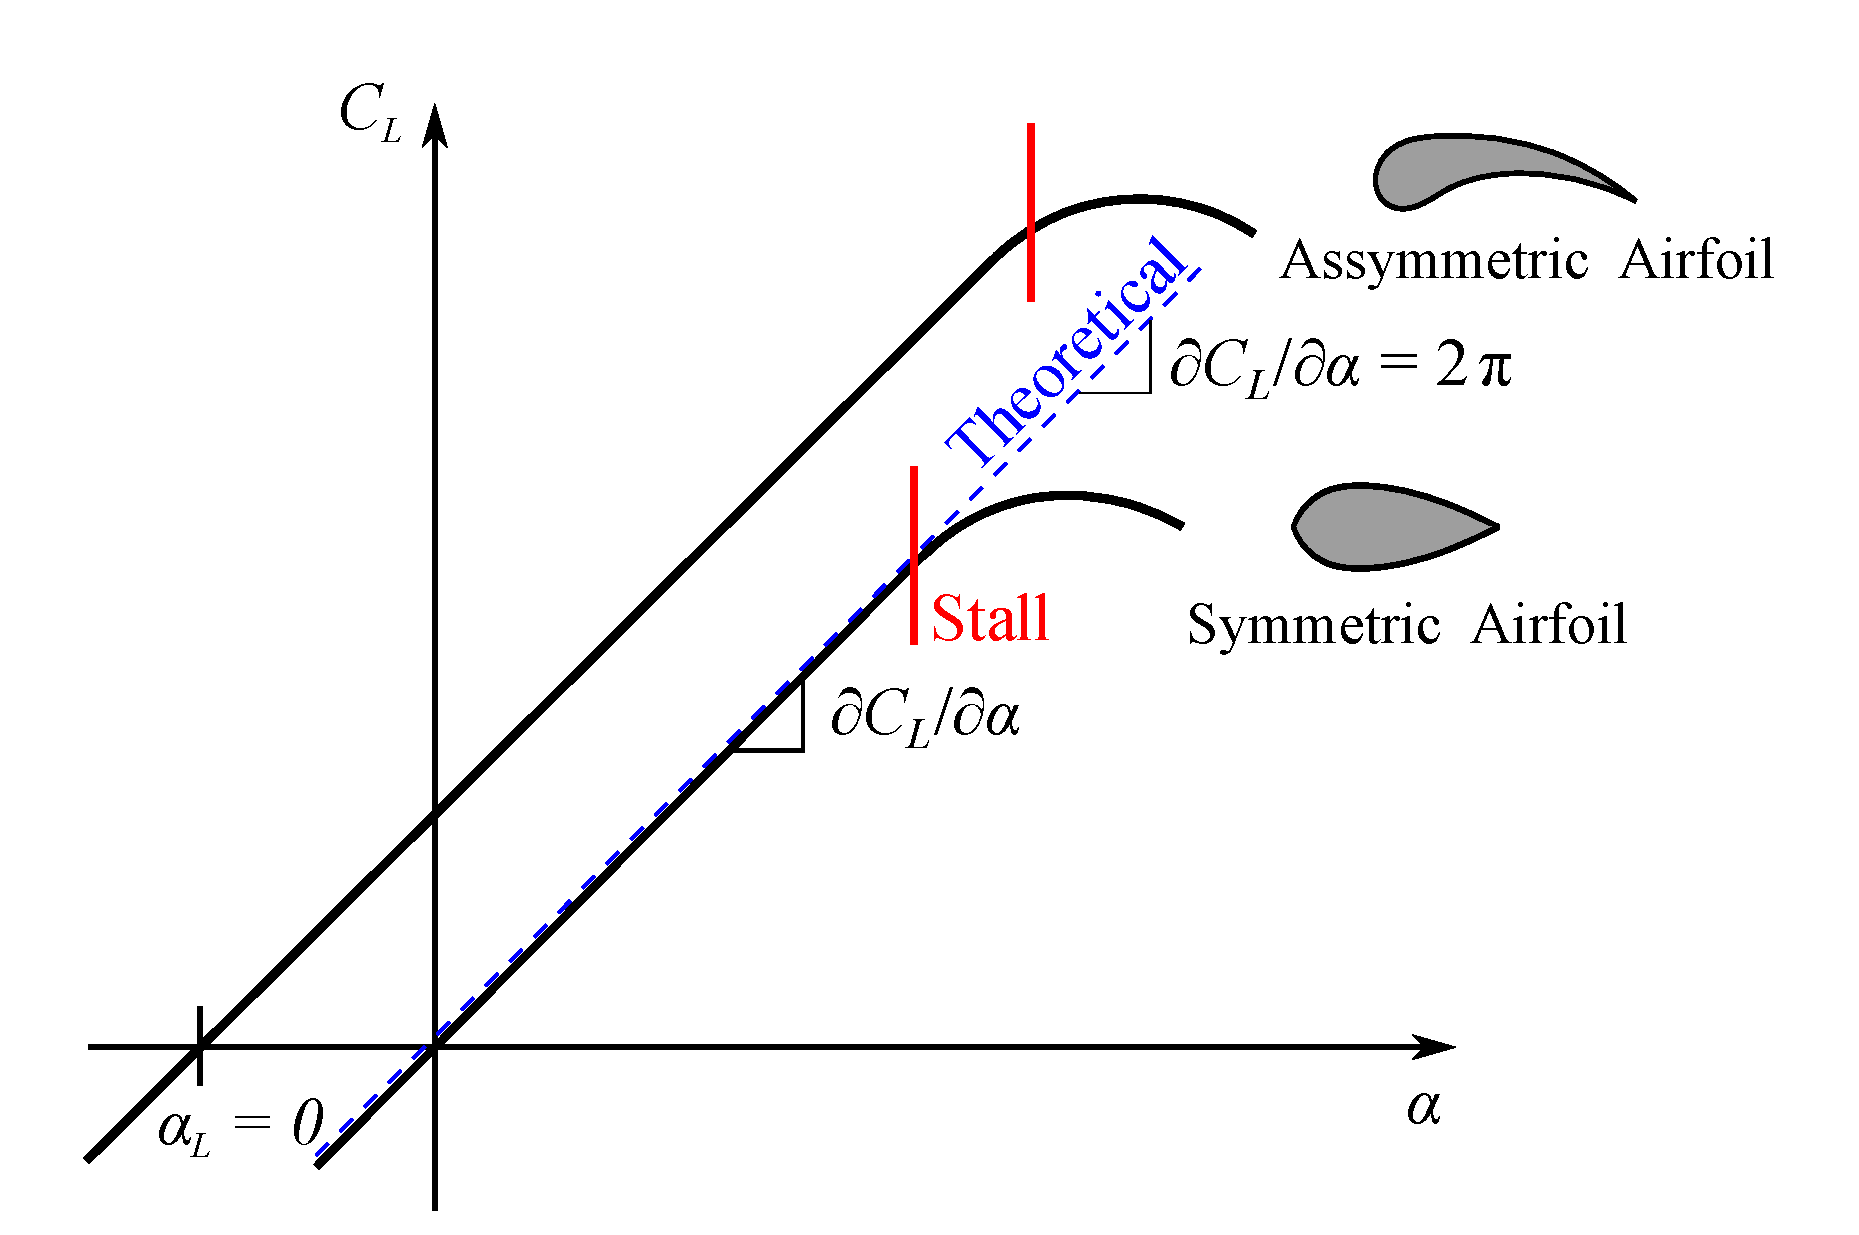
\includegraphics[width=0.68\textwidth]{liftCurve}
    \caption{\label{FIG_LIFT_CURVE}Airfoil lift curve.}
  \end{center}
\end{figure}
%================================================================

From thin airfoil theory \cite{ANDERSON_INTRO_TO_FLIGHT_BOOK2012} with the assumptions (i) $\M_\infty\ll 1$ and (ii) $\Re\to\infty$ (inviscid), we can relate the lift-coefficient to the angle of attack:
\begin{equation}
  c_l = a_0(\alpha-\alpha_0)\;,
\end{equation}
where
\begin{equation}
  a_0 = \f{\p c_l}{\p \alpha} = 2\pi \, \text{.}
\end{equation}

\begin{figure}[!h!]
  \begin{center}
    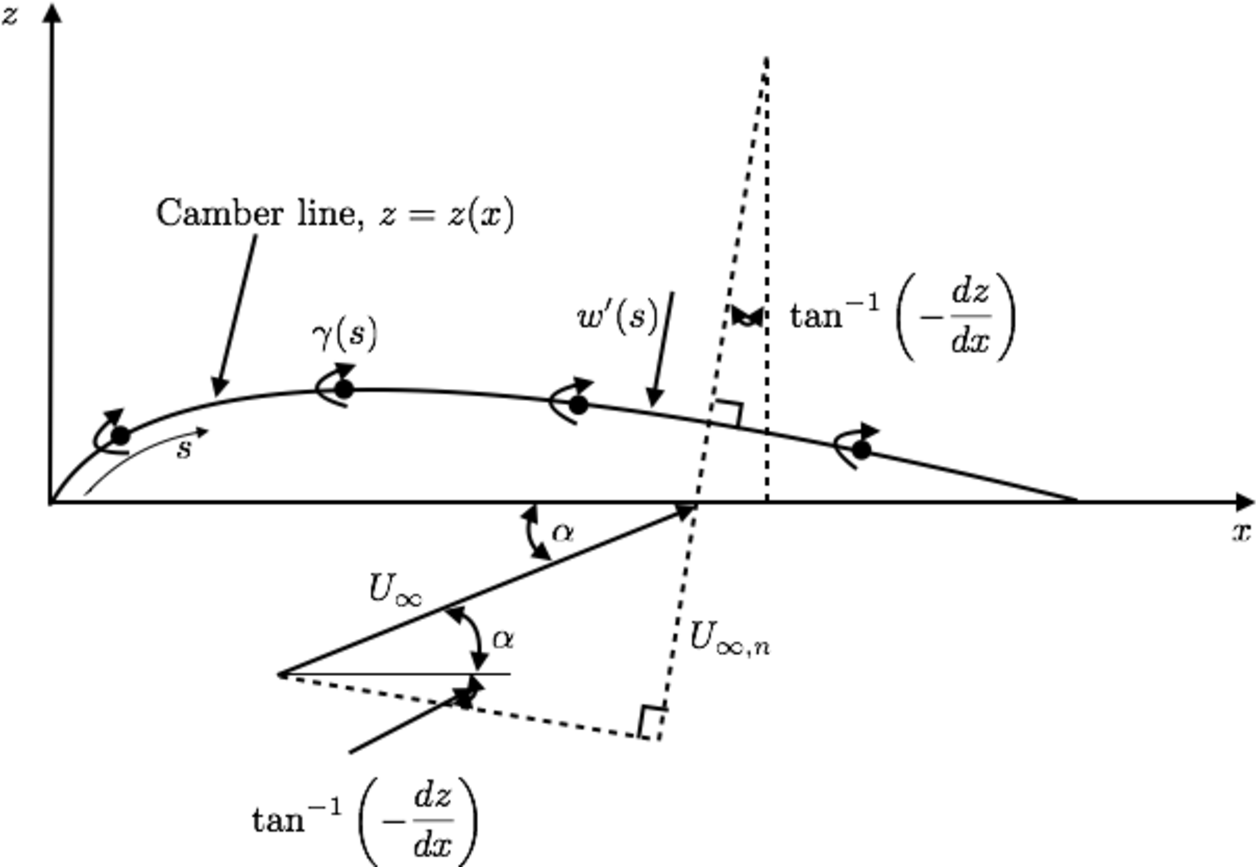
\includegraphics[width=0.68\textwidth]{thin_airfoil}
    \caption{\label{FIG_THIN_AIRFOIL}Thin airfoil and vortex sheet.}
  \end{center}
\end{figure}

\Cref{FIG_THIN_AIRFOIL} shows a thin airfoil with vortex sheet place along the camber line. The distance measured along the camber line is denoted by s. The shape of the camber line is given by $z = z(x)$. $U_\infty$ is the free stream velocity, with the angle of attack $\alpha$. $U_{\infty, n}$ and $w^\prime(s)$ are the velocity component normal to the camber line by the free stream and the vortext sheet respectively. Assuming that the camber line is a streamline, then
\begin{equation}
	U_{\infty, n} + w^\prime(s) = 0 \label{eq:camber_n}
\end{equation}
at every point along the camber line.

From the geometry, and assume the thin airfoil is at small angle of attack, $\tan^{-1}\left(-dz/dx\right)\approx-dz/dx$, we have
\begin{align}
	U_{\infty, n} &= U_\infty \sin \left[ \alpha + \tan^{-1}\left(-\frac{dz}{dx}\right)\right] \\
	&= U_\infty \left(\alpha - \frac{dz}{dx}\right). \label{eq:U_inf_n}
\end{align}

For a thin airfoil, the camber line is close to the chord line, thus $w^\prime(s)\approx w(x)$. The velocity $dw$ at piont $x$ induced by the elemental vortex at point $\xi$ is given as:
\begin{equation}
	dw = -\frac{\gamma(\xi)d\xi}{2\pi(x-\xi)}.
	\label{eq:dw}
\end{equation}
$w(x)$ can be obtained by integrating \cref{eq:dw} from the leading edge $\xi=0$ to the trialing edge $\xi=c$, which is
\begin{equation}
	w(x) = -\int_0^c\frac{\gamma(\xi)d\xi}{2\pi(x-\xi)}. \label{eq:wx}
\end{equation}

Substituting \cref{eq:U_inf_n,eq:wx} into \cref{eq:camber_n} yields the \emph{fundamental equation of thin airfoil theory}, which is
\begin{equation}
	\frac{1}{2\pi}\int_0^c\frac{\gamma(\xi)d\xi}{x-\xi}=U_\infty\left(\alpha-\frac{dz}{dx}\right). \label{eq:fund_eq_thin_airfoil}
\end{equation}
For a symmetric airfoil, $dz/dx=0$, and \cref{eq:fund_eq_thin_airfoil} becomes:
\begin{equation}
	\frac{1}{2\pi}\int_0^c\frac{\gamma(\xi)d\xi}{x-\xi}=U_\infty\alpha. \label{eq:fund_eq_thin_airfoil_sym}
\end{equation}
Introduce coordinate transformation
\begin{equation}
	\xi = \frac{c}{2}(1 - \cos \theta).
\end{equation}
Note that $x$ is a fixed point which corresponds to a particular value $\theta_0$, which is
\begin{equation}
	x = \frac{c}{2}(1 - \cos \theta_0).
\end{equation}
With this, \cref{eq:fund_eq_thin_airfoil_sym} becomes
\begin{equation}
	\frac{1}{2\pi}\int_0^\pi\frac{\gamma(\theta)\sin \theta d\theta}{\cos \theta - \cos \theta_0}=U_\infty\alpha. \label{eq:fund_eq_thin_airfoil_sym2}
\end{equation}
From the mathematical theory of integral equations,
\begin{equation}
	\gamma(\theta) = 2 \alpha U_\infty \frac{1 + \cos \theta}{\sin \theta}.
\end{equation}
Note that $\gamma(\theta)$ satisfies the Kutta condition
\begin{equation}
	\lim_{\theta\rightarrow\pi}\gamma(\theta)=2 \alpha U_\infty \frac{-\sin \pi}{\cos \pi} = 0.
\end{equation}
Integrating $\gamma(\xi)$ from $0$ to $c$ yields the total circulation around the airfoil, which is
\begin{align}
	\Gamma &= \int_0^c \gamma(\xi)d\xi \\
		&= \frac{c}{2}\int_0^\pi \gamma(\theta)\sin(\theta)d\theta \\
		&= \pi \alpha c U_\infty.
\end{align}
The lift per unit span is
\begin{equation}
	L = \rho_\infty U_\infty \Gamma = \pi \alpha c \rho_\infty U_\infty^2.
\end{equation}
The lift coefficient is then
\begin{equation}
	c_l = \frac{L}{q_\infty c} = \frac{\pi \alpha c \rho_\infty U_\infty^2}{\frac{1}{2}\rho_\infty U_\infty^2 c} = 2\pi \alpha.
\end{equation}
This yields the theoretical lift slope, which is
\begin{equation}
	a_0 = \frac{\partial c_l}{\partial \alpha} = 2\pi.
\end{equation}

The lift, drag and pressure-coefficients are typically obtained from measurements or computations of an ``infinite wing span'', meaning that there are no losses due to the  finite wing-span considered. To account for finite-wing effects due to the {\it induced drag} (i.e. pressure difference across wing tip and wing-tip vortices), we can separate the drag coefficient into two contributions:
\begin{equation}
  \label{EQ_CD_RELATION}
  \underbrace{C_D}_{\text{Total Drag}} = \underbrace{C_{D,0}}_{\text{Profile Drag}} + \underbrace{C_{D,i}}_{\text{Induced Drag}} \, \text{,}
\end{equation}
where the {\it profile drag} consists of contributions from (i) skin friction, (ii) pressure drag, and (iii) flow-separation. The downwash due to tip-vortex-generation contributes to the induced drag. Another induced-drag contribution, that we typically neglect in our analysis, is the {\it wave drag}, which becomes relevant for transonic and supersonic flight conditions. 
       
For the specific case of an elliptic lift distribution, we can employ Prandtl's lifting-line theory to find an analytic expression that relates $C_{D,i}$ to the lift coefficient:
\begin{equation}
  \label{EQ_CD_CL_RELATION}
  C_{D,i} = \f{C^2_L}{\pi e AR} \, \text{,}
\end{equation}
where the aspect ratio $AR$ is expressed in terms of the wing span $b$ and wing area $S$ as:
\begin{equation}
  AR = \f{b^2}{S}=\f{b}{c} \,,
\end{equation}
and the span efficiency factor is 
\begin{equation}
e = \begin{cases} 1 & \text{for elliptic lift distribution}\\
                             <1 & \text{for general case}
      \end{cases} \, \text{.}
\end{equation}
The derivation of \cref{EQ_CD_CL_RELATION} is out of the scope for this course. Readers who are interested in the derivation of this relation may refer to Chapter 5.3 in book \emph{Fundamentals of Aerodynamics} by J. Anderson for details. Upon inserting \cref{EQ_CD_CL_RELATION} into \cref{EQ_CD_RELATION} we can derive the so-called {\it drag polar}:
\begin{equation}
C_D = C_{D,0} + \f{C^2_L}{\pi e AR} \, \text{,}
\end{equation}
which provides a relation between lift, profile drag, and total drag acting on an airfoil. A schematic of the drag polar is shown in \cref{FIG_DRAG_POLAR}.

%================================================================
\begin{figure}[!h!]
\begin{center}
 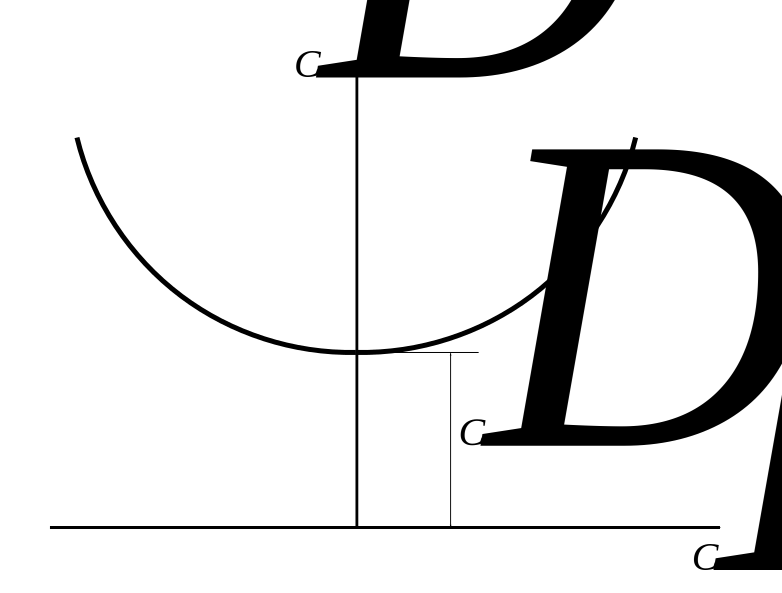
\includegraphics[width=0.46\textwidth]{dragPolar}
 \caption{\label{FIG_DRAG_POLAR}Drag polar.}
\end{center}
\end{figure}
%================================================================

%%%%%%%%%%%%%%%%%%%%%%%%%%%%%%%%%%%%%%%%%%%%%%%%%%%%%%%%%%%%%%%%%
\subsection{Aircraft Performance}
%%%%%%%%%%%%%%%%%%%%%%%%%%%%%%%%%%%%%%%%%%%%%%%%%%%%%%%%%%%%%%%%%

%%%%%%%%%%%%%%%%%%%%%%%%%%%%%%%%%%%%%%%%%%%%%%%%%%%%%%%%%%%%%%%%%
\subsubsection{Extension of Lift and Drag Coefficients}
%%%%%%%%%%%%%%%%%%%%%%%%%%%%%%%%%%%%%%%%%%%%%%%%%%%%%%%%%%%%%%%%%
This section extends the aerodynamic analysis that we performed by considering an isolated airfoil to the entire aircraft. For this, we are including additional effects and contributions due to lift and drag, arising from the airfoil, fuselage, tail flaps, landing gear, and nacelle by extending the notion of $C_D$ and $C_L$. Following this spirit, we now define $C_L$ as the {\it total lift coefficient} (that includes contributions from the above-mentioned components). The drag-coefficient of the complete aircraft is then defined as
\begin{equation}
  \label{EQ_DRAG_POLAR_AIRCRAFT}
  C_D = C_{D,0} + \f{C^2_L}{\pi e AR}
\end{equation}
where $C_{D,0}$ is the zero-lift drag coefficient of the entire aircraft (see \cref{FIG_DRAG_POLAR}), and $e$ is the Oswald efficiency factor.

The resulting drag polar of the aircraft is shown in \cref{FIG_DRAG_POLAR_AIRCRAFT}.

%================================================================
\begin{figure}[!h!]
  \begin{center}
    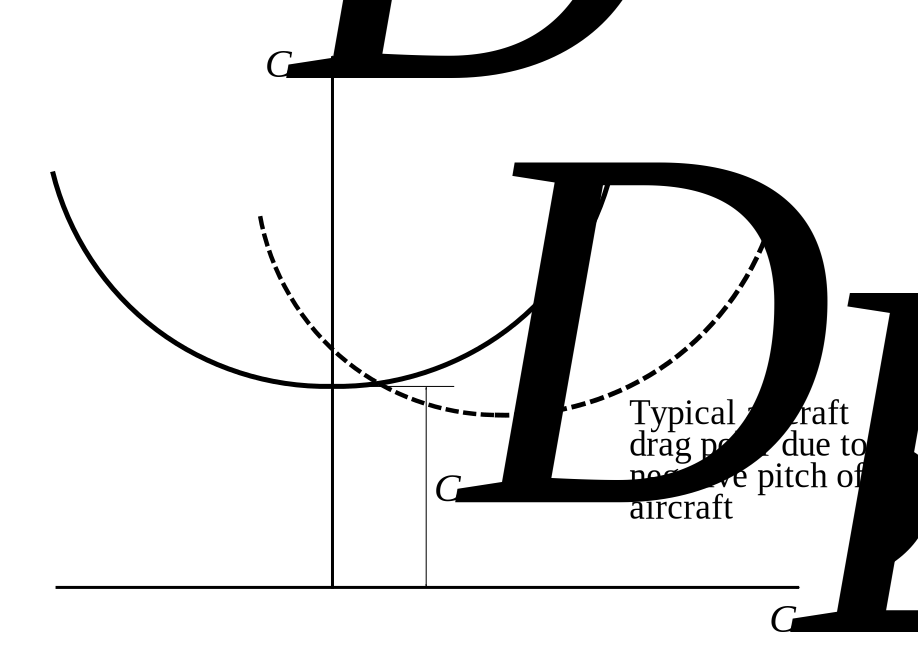
\includegraphics[width=0.56\textwidth]{dragPolarAircraft}
    \caption{\label{FIG_DRAG_POLAR_AIRCRAFT}Drag polar of aircraft, defined by \cref{EQ_DRAG_POLAR_AIRCRAFT}. Note that the minimum drag coefficient is shifted to $C_L>0$, since the zero-lift angle, $\alpha_{L=0}$, is often negative due to the downward pitch of the aircraft (a good example for this can be seen by the titled engines on an MD-80). Although rarely considered, lift is also generated at negative $C_L$ due to the fact that $\alpha_{L=0}<0$.}
  \end{center}
\end{figure}
%================================================================

%%%%%%%%%%%%%%%%%%%%%%%%%%%%%%%%%%%%%%%%%%%%%%%%%%%%%%%%%%%%%%%%%
\subsubsection{Force Balance and Thrust Requirements}
%%%%%%%%%%%%%%%%%%%%%%%%%%%%%%%%%%%%%%%%%%%%%%%%%%%%%%%%%%%%%%%%%

%================================================================
\begin{figure}[!h!]
  \begin{center}
    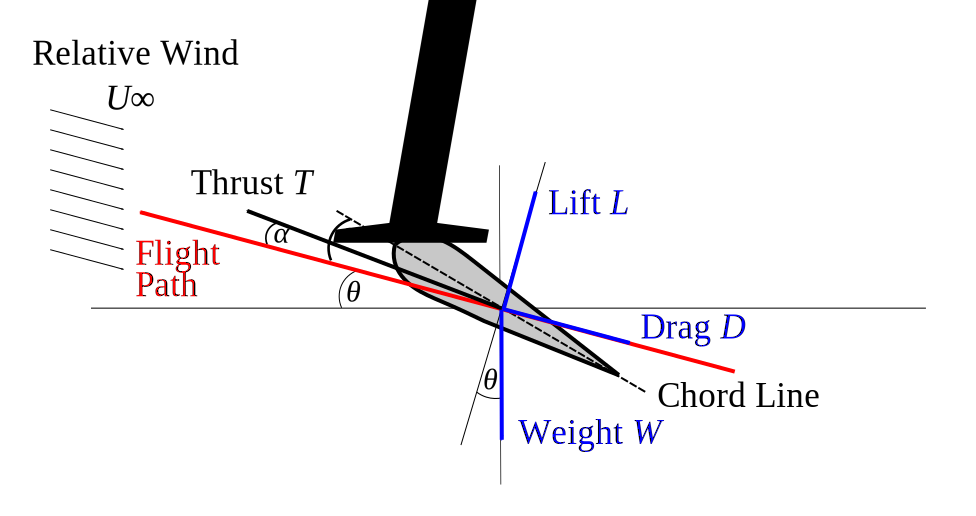
\includegraphics[width=0.7\textwidth]{forceBalanceAirfoil}
    \caption{\label{FIG_FORCE_BALANCE_AIRCRAFT}Force balance on aircraft with $\alpha$: angle-of-attack; $\theta$: inclination angle of flight path with respect to horizontal; $\alpha_T$: thrust-angle; $W$: weight; $L$: lift (perpendicular to flight path); $D$: drag (parallel to flight path); and $T$: thrust.}
  \end{center}
\end{figure}
%================================================================

From the force balance on an aircraft (see \cref{FIG_FORCE_BALANCE_AIRCRAFT}) we can set up the {\it force balance parallel to the flight path}:
\begin{equation}
   \sum_i F^\parallel_i = m\f{dU}{dt}\quad \Rightarrow\quad T\cos\alpha_T - W\sin\theta -D = m\f{dU}{dt} \, \text{,}
\end{equation}
and the {\it force balance perpendicular to the flight path}:
\begin{equation}
  \sum_i F^\perp_i = m\f{U^2}{r_c}\quad \Rightarrow\quad L+T\sin\alpha_T-W\cos\theta = m\f{U^2}{r_c} \, \text{,}
\end{equation}
where $r_c$ is the radius of the flight path (inverse of curvature of flight path).

We have some remarks and simplifications of the force balance equations:
\begin{itemize}[noitemsep,topsep=2pt]
   \item Note that $m=m(t)$, since we consume fuel during the flight:
   \begin{equation}
     m(t) = m_0 - \int_0^t \dot{m}_{fuel} dt \, \text{;}
   \end{equation}
   \item Since $\dot{m}_{fuel}$ is typically small compared to the airframe mass for airbreathing propulsion systems, we can typically neglect these effects;
   \item Often we can invoke the following sequence of simplifications:
     \begin{enumerate}[label=(\alph*),noitemsep,topsep=2pt]
       \item For the case of steady-state flight conditions, we have $d_tU = dU/dt = 0:$
         \begin{subeqnarray}
           T\cos\alpha_T - W\sin\theta -D &=& 0\\
           L+T\sin\alpha_T-W\cos\theta &=& m\f{U^2}{r_c}
         \end{subeqnarray}
       \item Thrust vector aligned with flight path ($\alpha_T=0$)
         \begin{subeqnarray}
           T - W\sin\theta -D &=& 0\\
           L-W\cos\theta &=& m\f{U^2}{r_c}
         \end{subeqnarray}
       \item Level flight: $r_c\to \infty; \theta = 0$
         \begin{subeqnarray}
           T -D &=& 0\\
           L-W &=& 0
         \end{subeqnarray}
      This reduced set of force-balance equations will be the basis for the subsequent analysis. If necessary individual assumptions can be relaxed to introduce more complexity.
      \end{enumerate}
\end{itemize}

The thrust and lift requirements for steady-level flight are:
\begin{subeqnarray}
  T = D = C_Dq_\infty S\phantom{\, \text{.}}\\
  L = W = C_Lq_\infty S\, \text{.}
\end{subeqnarray}
By taking the ratio of both equations, we have an expression for the {\it required thrust}:
\begin{equation}
  T^\ast = W\f{D}{L} = W\f{C_D}{C_L} \, \text{,}
\end{equation}
and with the  drag polar from \cref{EQ_DRAG_POLAR_AIRCRAFT}, we can write:
\begin{equation}
  T^\ast = \underbrace{C_{D,0}q_\infty S}_{\text{zero-lift drag}} + \underbrace{\f{W^2}{q_\infty S\pi e AR}}_{\text{lift-induced drag}} \, \text{.}
\end{equation}
The required thrust and thrust components vs. dynamic pressure are illustrated in \cref{FIG_THRUST_REQUIREMENT}. 

%================================================================
\begin{figure}[!b!]
\begin{center}
 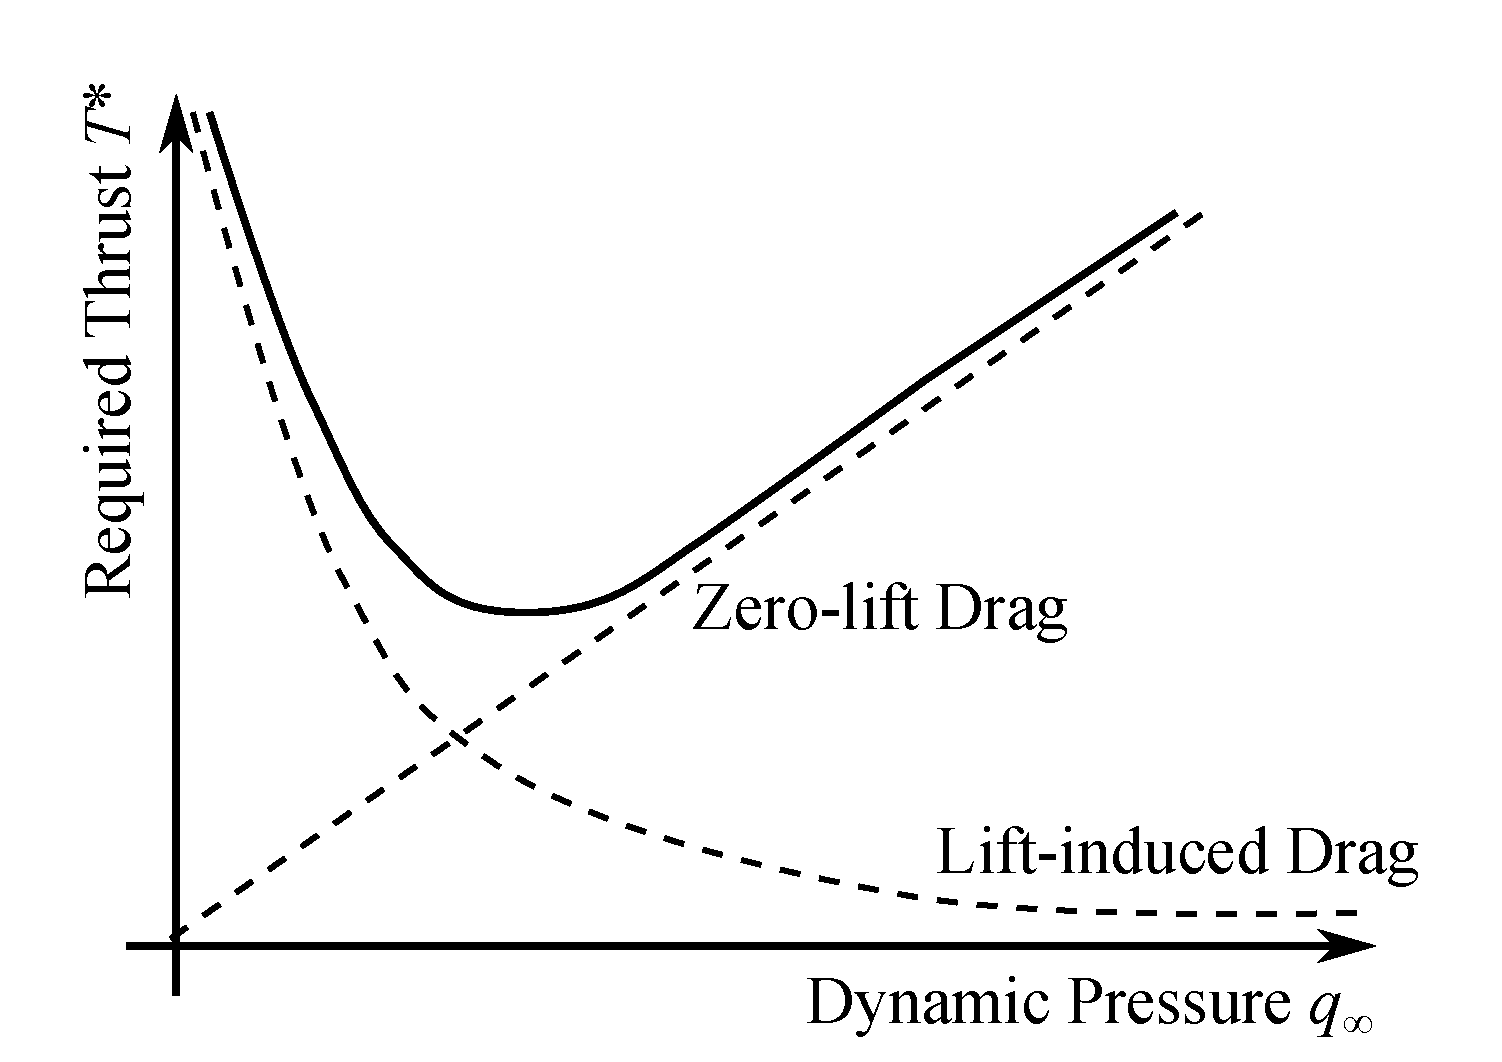
\includegraphics[width=0.55\textwidth]{requiredThrustVsDynamicPressure}
 \caption{\label{FIG_THRUST_REQUIREMENT}Required thrust vs. dynamic pressure.}
\end{center}
\end{figure}
%================================================================
 
The dependence of the thrust requirements on the angle of attack can be reconciled by introducing the expression for $C_L$ from thin airfoil theory, $C_L = a(\alpha-\alpha_0) = 2\pi (\alpha-\alpha_0)$, into the thrust equation:
\begin{equation}
  T^\ast = C_{D,0}q_\infty S + \f{[2\pi(\alpha-\alpha_0)]^2q_\infty S}{\pi e AR} \, \text{.}
\end{equation}

%%%%%%%%%%%%%%%%%%%%%%%%%%%%%%%%%%%%%%%%%%%%%%%%%%%%%%%%%%%%%%%%%
\subsubsection{Available Thrust}
%%%%%%%%%%%%%%%%%%%%%%%%%%%%%%%%%%%%%%%%%%%%%%%%%%%%%%%%%%%%%%%%%
The thrust that is provided by the engine (propeller-driven IC-engine and gas turbine, etc.) must match or exceed the required thrust. We will see later that different propulsion systems have different thrust characteristics and limitations (see \cref{FIG_THRUST_REQUIREMENT_AVAIL}) and the maximum flight speed and cruise altitude is then determined by the available thrust of the aircraft.

Note that while gas-turbines are typically rated by thrust, the performance of IC-engines is typically specified in terms of power; required flight power and thrust are related through the following expression:
\begin{equation}
  P^\ast = T^\ast U_\infty \, \text{.}
\end{equation}

%================================================================
\begin{figure}[htb]
  \begin{center}
    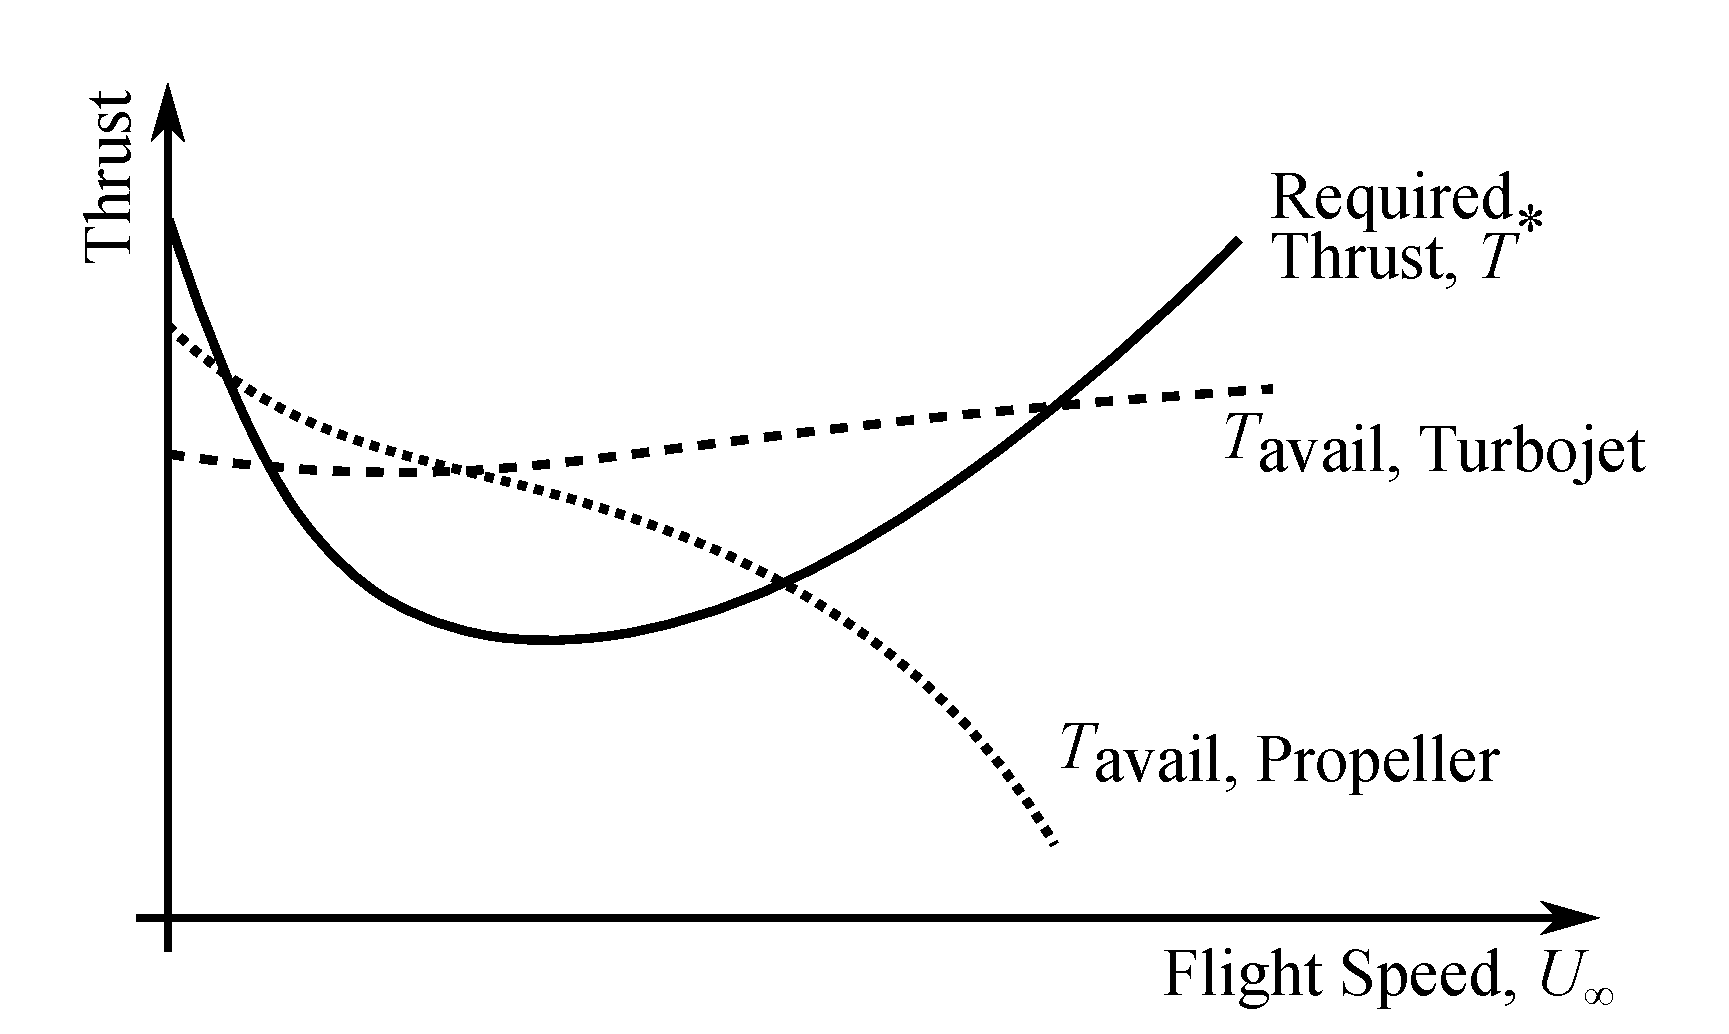
\includegraphics[width=0.56\textwidth]{thrustRequirements}
    \caption{\label{FIG_THRUST_REQUIREMENT_AVAIL}Comparison of required and available thrust for different propulsion systems.}
  \end{center}
\end{figure}
%================================================================

%%%%%%%%%%%%%%%%%%%%%%%%%%%%%%%%%%%%%%%%%%%%%%%%%%%%%%%%%%%%%%%%%
\subsection{Propulsive Thrust Generation}
%%%%%%%%%%%%%%%%%%%%%%%%%%%%%%%%%%%%%%%%%%%%%%%%%%%%%%%%%%%%%%%%%
Recall from previous sections that the required thrust is a function of speed $U_\infty$, angle of attack $\alpha$, and other flight parameters. For steady flight we  found
\begin{equation}
  \text{Required Thrust:}\quad T^\ast = C_{D,0}q_\infty S + \f{W^2}{q_\infty S \pi e AR} \, \text{.}
\end{equation}
The required thrust must be matched or exceeded by the available thrust to meet the performance requirement. The objective now is to link the required thrust to the engine thrust. For this we consider two propulsion systems, namely gas-turbine engine and propeller-driven engine (with relevance to turbofan engine).

%%%%%%%%%%%%%%%%%%%%%%%%%%%%%%%%%%%%%%%%%%%%%%%%%%%%%%%%%%%%%%%%%
\subsubsection{Thrust Equation}
%%%%%%%%%%%%%%%%%%%%%%%%%%%%%%%%%%%%%%%%%%%%%%%%%%%%%%%%%%%%%%%%%
A general equation for the thrust of airbreathing propulsion (and with some minor modifications also for rocket engines) can be derived from the conservation equations for mass and momentum. For this analysis we consider a control-volume in the coordinate system that is fixed to the engine (see \cref{FIG_CV_ANALYSIS}).

%================================================================
\begin{figure}[!h!]
\begin{center}
 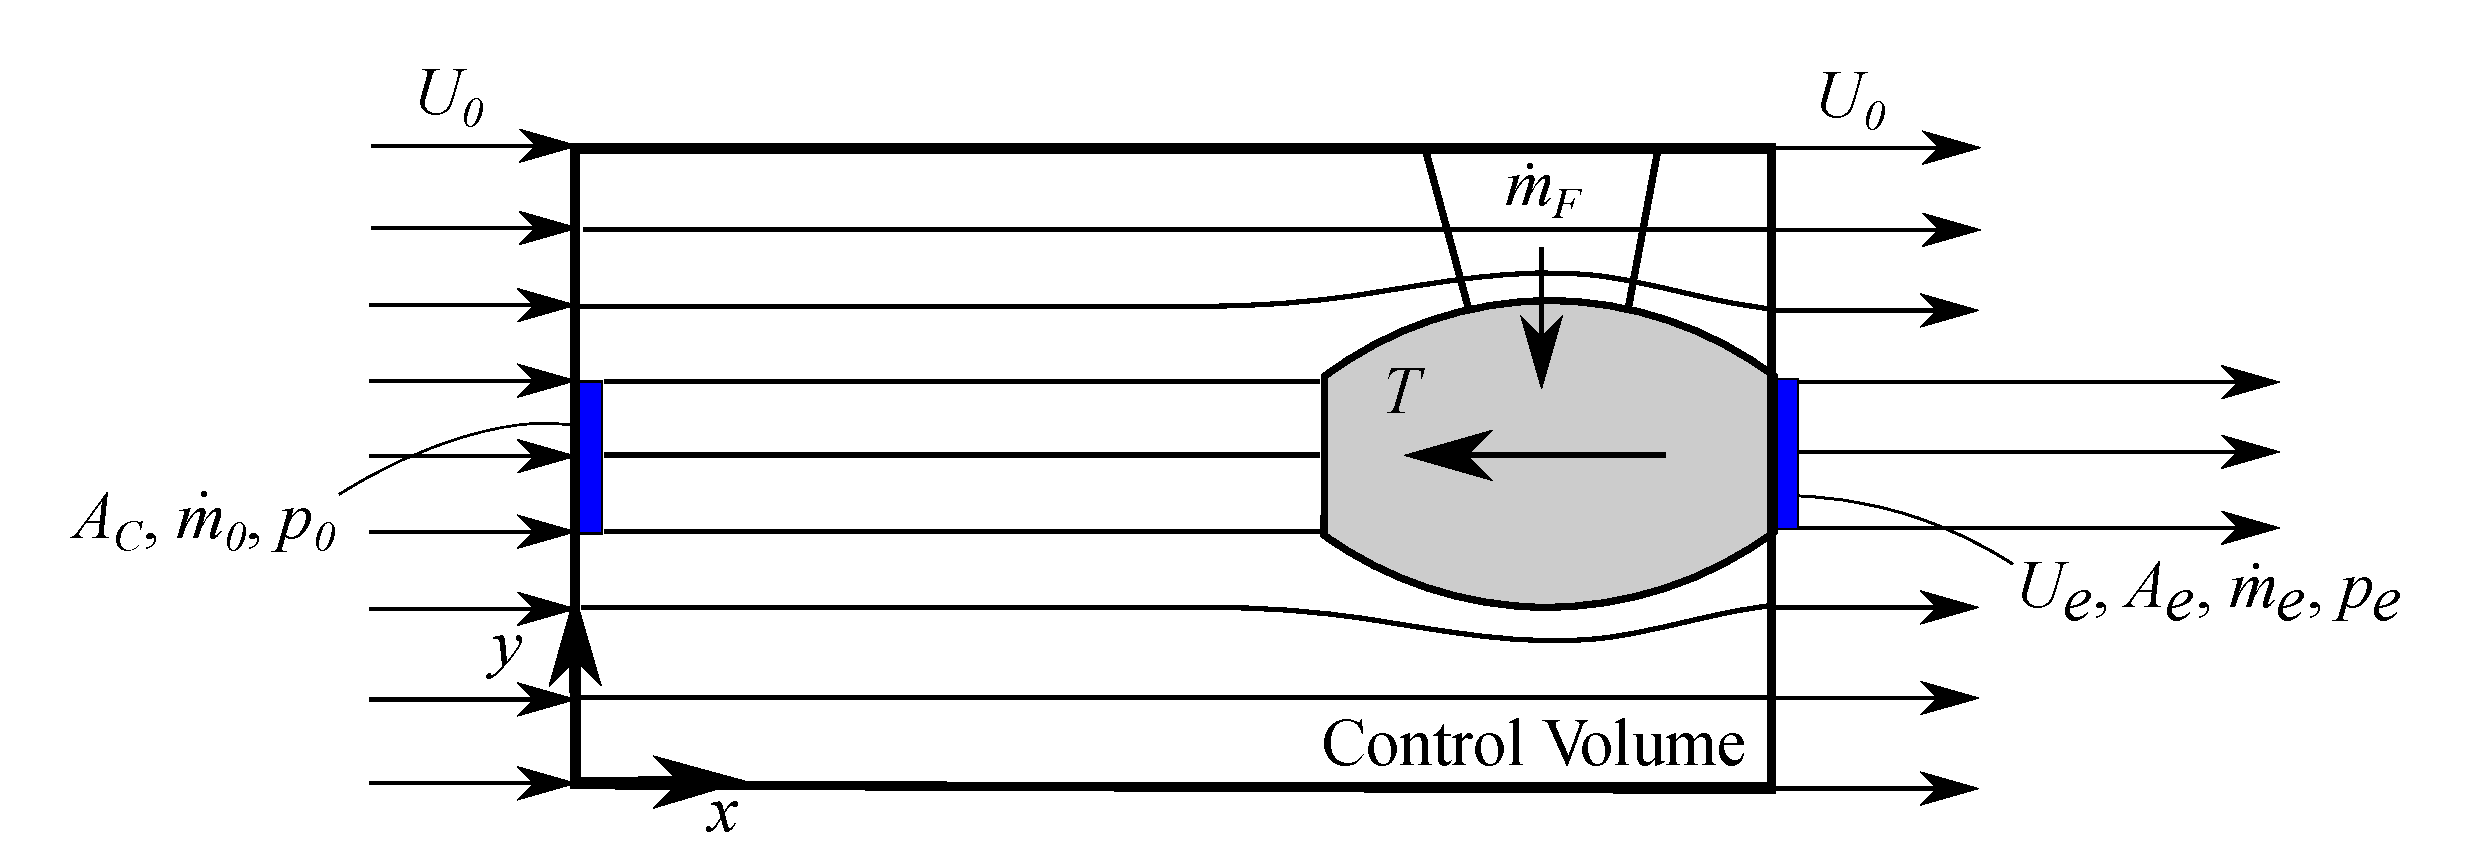
\includegraphics[width=0.88\textwidth]{thrustEquationCV}
 \caption{\label{FIG_CV_ANALYSIS}Control volume analysis for thrust equation.}
\end{center}
\end{figure}
%================================================================

Recall conservation equations
\begin{subeqnarray}
  \text{Mass:} &  \underbrace{\p_t \rho}_{\text{Rate of change}} +  \underbrace{\nabla\cdot(\rho \uvec)}_{\text{Flux of mass}} = 0\\
  \text{Momentum:} & \underbrace{\p_t (\rho\uvec)}_{\text{Rate of change}} + \underbrace{\nabla\cdot(\rho\uvec\otimes\uvec)}_{\text{Flux of momentum}} = \underbrace{-\nabla p}_{\text{Pressure force}} + \underbrace{\nabla\cdot \sigmamat}_{\text{Viscous force}} + \underbrace{\gvec}_{\text{Gravity}} + \underbrace{\fvec}_{\text{Reaction force}}
\end{subeqnarray} 
and integrate over control-volume with $d \svec$ defined to be the outward-pointing surface element
\begin{equation}
d \svec = |d\svec| \hat{\nvec} = ds \,\hat{\nvec} \, ,
\end{equation}
we will have the following form (by using the Gauss theorem):
\begin{subeqnarray}
  \p_t \int \rho dV + \oint (\rho \uvec)\cdot\wh\nvec \,d s&=& 0 \, \text{,}\\
  \p_t \int (\rho \uvec) dV + \oint(\rho \uvec) (\uvec\cdot\wh{\nvec})d s &=& - \oint p \wh\nvec\, ds + \oint \sigmamat \cdot \wh\nvec \,ds +  \int \gvec dV + \Fvec \, \text{,}
\end{subeqnarray} 
where $\Fvec = \int \fvec dV$ is the reaction force. By introducing the following assumptions:
\begin{itemizePacked}
  \item Steady state;
  \item Negligible viscous effects;
  \item Negligible gravitational forces (might become relevant for rocket-engines);
  \item Constant flow rates/properties across area cross-sections;
  \item Assume that thrust is aligned with $x$-direction,
\end{itemizePacked}
we can obtain the steady-state conservation equations for mass and momentum:
\begin{subeqnarray}
  \oint (\rho \uvec)\cdot\wh\nvec d s&=& 0 \, \text{,}\\
  \oint(\rho u_x) \uvec\cdot\wh{\nvec}d s + \oint p d S_x &=& F_x = T_U \, \text{,}
\end{subeqnarray} 
where $T_U$ is named the uninstalled thrust. By assuming that all flow-field quantities are piece-wise constant at each area-section, we can reduce the integral equations to algebraic equations:
\begin{subeqnarray}
  \text{Mass:} & -\rho_0 U_0 A_C  + \rho_eU_eA_e - \dot{m}_{F} = 0\\
  \text{$x$-Momentum:} & -\rho_0 U^2_0 A_C - p_0 A_e + \rho_e U^2_e A_e +p_e A_e = F_x
\end{subeqnarray}
and with
\begin{eqnarray}
  \dot{m}_e &=& \rho_eU_eA_e\, ,\\
  \dot{m}_A &=& \rho_0 U_0 A_C\, ,
\end{eqnarray}
where $\dot{m}_A$ is the air mass flow, we have 
\begin{subeqnarray}
\dot{m}_e = \dot{m}_A + \dot{m}_F = \dot{m}_A \left(1+\frac{\dot{m}_F}{\dot{m}_A} \right) \, , \\
F_x = \dot{m}_e U_e + \dot{m}_A U_0 + A_e (p_e - p_0) \, ,
\end{subeqnarray}
and hence we obtain the thrust equation
\begin{equation}
  \label{EQ_THRUST_EQUATION}
  F_x = T_U = \underbrace{\dot{m}_A \left[ \left(1+\f{\dot{m}_F}{\dot{m}_A}\right)U_e - U_0\right]}_{\text{Jet thrust}} + \underbrace{A_e\left(p_e - p_0\right)}_{\text{Pressure thrust}} \, \text{.}
\end{equation}

We have several remarks:
\begin{itemizePacked}
  \item Pressure thrust is typically small (zero) for subsonic aircraft and perfect expansion nozzle ($p_e = p_0$), and requires consideration for rockets and imperfectly expanded nozzles.
  \item By applying the thrust equation to propeller-flows with $\dot{m}_{F}=0$ and $p_e = p_0$, we have:
    \begin{equation}
      T_{\text{Prop}} = \dot{m}_A(U_e - U_0) \, \text{;}
    \end{equation}
  \item Applied to rockets ($\dot{m}_A = 0$) we have
   \begin{eqnarray}
     T_{\text{Rocket}} = \dot{m}_p U_e + {A_e\left(p_e - p_0\right)} \, \text{,}
   \end{eqnarray}
   where $\dot{m}_p$ is the mass flow rate of propellant.
  \item Often thrust equation derived above is referred to as {\it uninstalled thrust}, since it neglects the effects due to inlet drag and nozzle drag:
  \begin{eqnarray}
     T_I = T_U - D_{\text{Inlet}} - D_{\text{Nozzle}} \, \text{,}
  \end{eqnarray}
  where $T_I$ is the installed thrust, and the inlet and nozzle drag coefficients are defined as
  \begin{eqnarray}
     \phi_\text{Inlet} &=& \frac{D_\text{Inlet}}{T_u} \sim 0.02-0.5 \, \text{,}\\
     \phi_\text{Nozzle} &=& \frac{D_\text{Nozzle}}{T_u} \sim 0.01 \, \text{,}
  \end{eqnarray}
  and we can write
    \begin{eqnarray}
     T_I = T_U (1- \phi_{\text{Inlet}} - \phi_{\text{Nozzle}}) \, \text{.}
  \end{eqnarray} 
  \item Often thrust is given in English units,
    \begin{equation}
    T = T g_c \quad \text{and} \quad g_c = \left\{ 
         \begin{array}{r@{,\quad}l}
          1 & {\text{SI metric}}\\
          32.17 & {\frac{\text{lbm}\cdot\text{ft}}{\text{lbf}\cdot\text{s}^2}}\\
         \end{array}
         \right. \, \text{,}
    \end{equation}
    where lbm is pound mass and lbf is pound force. For $g_c$, since 1 N = 0.22482 lbf, 1~m~=~3.2808~ft and 1 kg = 2.2046 lbm, we have
    \begin{equation}
    g_c = \frac{\text{kg}\cdot\text{m}}{\text{s}^2\cdot\text{N}} = 1 = \frac{(2.2046\text{lbm})(3.2808\text{ft})}{\text{s}^2(0.22482\text{lbf})} = 32.17\, \frac{\text{lbm}\cdot\text{ft}}{\text{lbf}\cdot\text{s}^2} \, .
    \end{equation}
\end{itemizePacked}

%%%%%%%%%%%%%%%%%%%%%%%%%%%%%%%%%%%%%%%%%%%%%%%%%%%%%%%%%%%%%%%%%
\subsubsection{Thrust Equation for Turbofan Engines}
%%%%%%%%%%%%%%%%%%%%%%%%%%%%%%%%%%%%%%%%%%%%%%%%%%%%%%%%%%%%%%%%%
Classic thrust equation that we derived above only considers a single stream through the engine. However, for turbofan engines, the air stream is split into two separated streams \textendash one going through the core and the other one passing by (``bypass") and generating thrust by airflow acceleration. 

\Cref{FIG_STATION_NUMBERING} shows the control volume and definitions of the stations in a turbofan engine. Abbreviations are LPC for low-pressure compressor, HPC for high-pressure compressor, LPT for low-pressure turbine, and HPT for high-pressure turbine. Note that stations 6 and 7 are omitted and correspond to the combustor inlet/exit of the afterburner.

The bypass ratio is defined as
\begin{equation}
\beta = \frac{\dot{m}_{A\,,B}}{\dot{m}_{A\,,C}} \,,
\end{equation}
where $\dot{m}_{A\,,B}$ is the airflow through bypass and $\dot{m}_{A\,,C}$ is the airflow through core.

Assume that both streams expand to $p_e = p_0$ separately and there is no mixing among streams. Thrust equation for turbofan engine in general form is
\begin{equation}
  T = \dot{m}_{A\,,C} \left[ (1+f) U_e + \beta U_{1e} - (1+\beta) U_0 \right] + A_e (p_e - p_0) + A_{1e} (p_{1e} - p_0)\, \text{,}
\end{equation}
where $f = \dot{m}_F/\dot{m}_A$, $U_e$ is the core exit velocity, and $U_{1e}$ is the fan exit velocity.

%==============================================================
\begin{figure}[!htb!]
 \centering
    {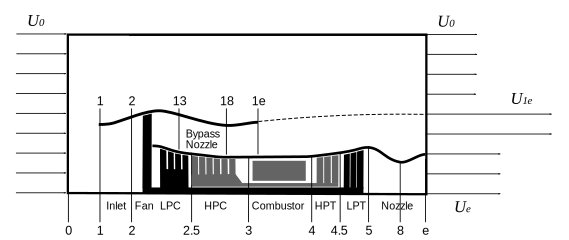
\includegraphics[width=0.9\textwidth, clip=, keepaspectratio]{turboFanEngine}}
    \caption{\label{FIG_STATION_NUMBERING}Control volume analysis for turbofan thrust equation and station numbering for a commercial twin-spool turbofan engine.}
\end{figure}
%==============================================================

%%%%%%%%%%%%%%%%%%%%%%%%%%%%%%%%%%%%%%%%%%%%%%%%%%%%%%%%%%%%%%%%%
\subsection{Fuel Consumption and Range Equation}
%%%%%%%%%%%%%%%%%%%%%%%%%%%%%%%%%%%%%%%%%%%%%%%%%%%%%%%%%%%%%%%%%
The weight of the aircraft decreases during the flight as a result of the fuel consumption. The aircraft mass can be expressed as
\begin{equation}
  m = \underbrace{m_{AF}}_{\text{Airframe mass}} + \underbrace{m_F}_{\text{Fuel mass}} \, ,
\end{equation}
where $m_{AF}$ is fixed and 
\begin{equation}
  m_F = m_{F, 0} - \int_0^t \dot{m}_F dt
\end{equation}
in which $\dot{m}_F$ is the fuel consumption rate and $m_{F,0}$ is the initial fuel mass. The rate of change of the weight of the aircraft, $W = mg$, is
\begin{equation}
  \frac{dW}{dt} = \frac{d}{dt}(mg) = - \dot{m}_F g \, .
\end{equation}
With the {\it thrust specific fuel consumption} defined as
\begin{equation}
  \text{TSFC} = \frac{\dot{m}_F}{T}
\end{equation}
where $T$ is the thrust, we have
\begin{equation}
  \frac{dW}{dt} = - \text{TFSC}\, T g\,.
\end{equation}
For level flight, we have $T = W (C_D/C_L)$ and thus
\begin{equation}
  \frac{dW}{W} = - \text{TSFC} \, \frac{C_D}{C_L} g dt\,.
\end{equation}
With the {\it endurance factor} EF defined as
\begin{equation}
\text{EF} = \frac{C_L}{C_D} \frac{1}{\text{TSFC} \,g}\,,
\end{equation}
we have 
\begin{equation}
\frac{dW}{W} = -\frac{dt}{\text{EF}}\,.
\end{equation}

Assume $C_D/C_L$ is constant, we can integrate to have the weight as a function of flight time,
\begin{equation}
  \frac{W(t)}{W_0} = \text{exp}\left(-\frac{t}{\text{EF}}\right) = \text{exp}\left(-\frac{C_D}{C_L} \text{TSFC} \, g \,t\right) \,.
\end{equation}
By using $ds = U dt$ and the {\it range factor} RF defined as 
\begin{equation}
\text{RF} = \frac{C_L}{C_D} \frac{U}{\text{TSFC} \,g}\,,
\end{equation}
we have
\begin{equation}
  \label{eqn:BRE}
  \frac{W(s)}{W_0} = \text{exp}\left(-\frac{s}{\text{RF}}\right) = \text{exp}\left(-\frac{C_D}{C_L} \frac{\text{TSFC}}{U} \, g \,s\right) \,.
\end{equation}
\Cref{eqn:BRE} is referred to as the Breguet range equation. \Cref{fig:EFRF} shows the plots of EF and RF as a function of flight Mach number and the flying altitude.

%================================================================
\begin{figure}[!b!]
  \begin{center}
    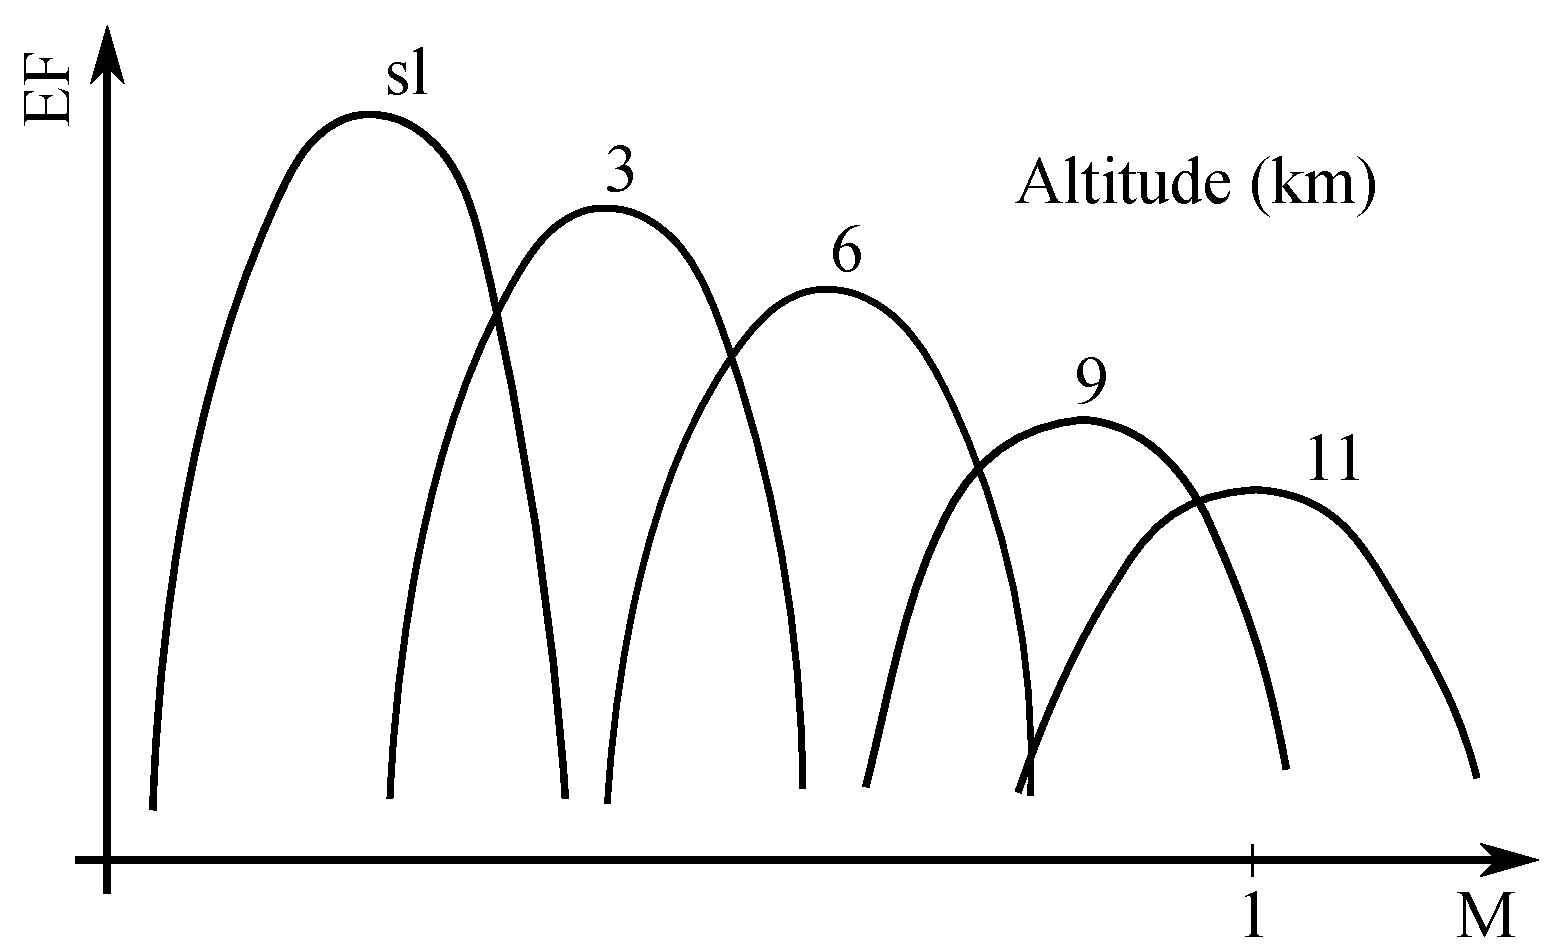
\includegraphics[width=0.48\textwidth]{EF}
    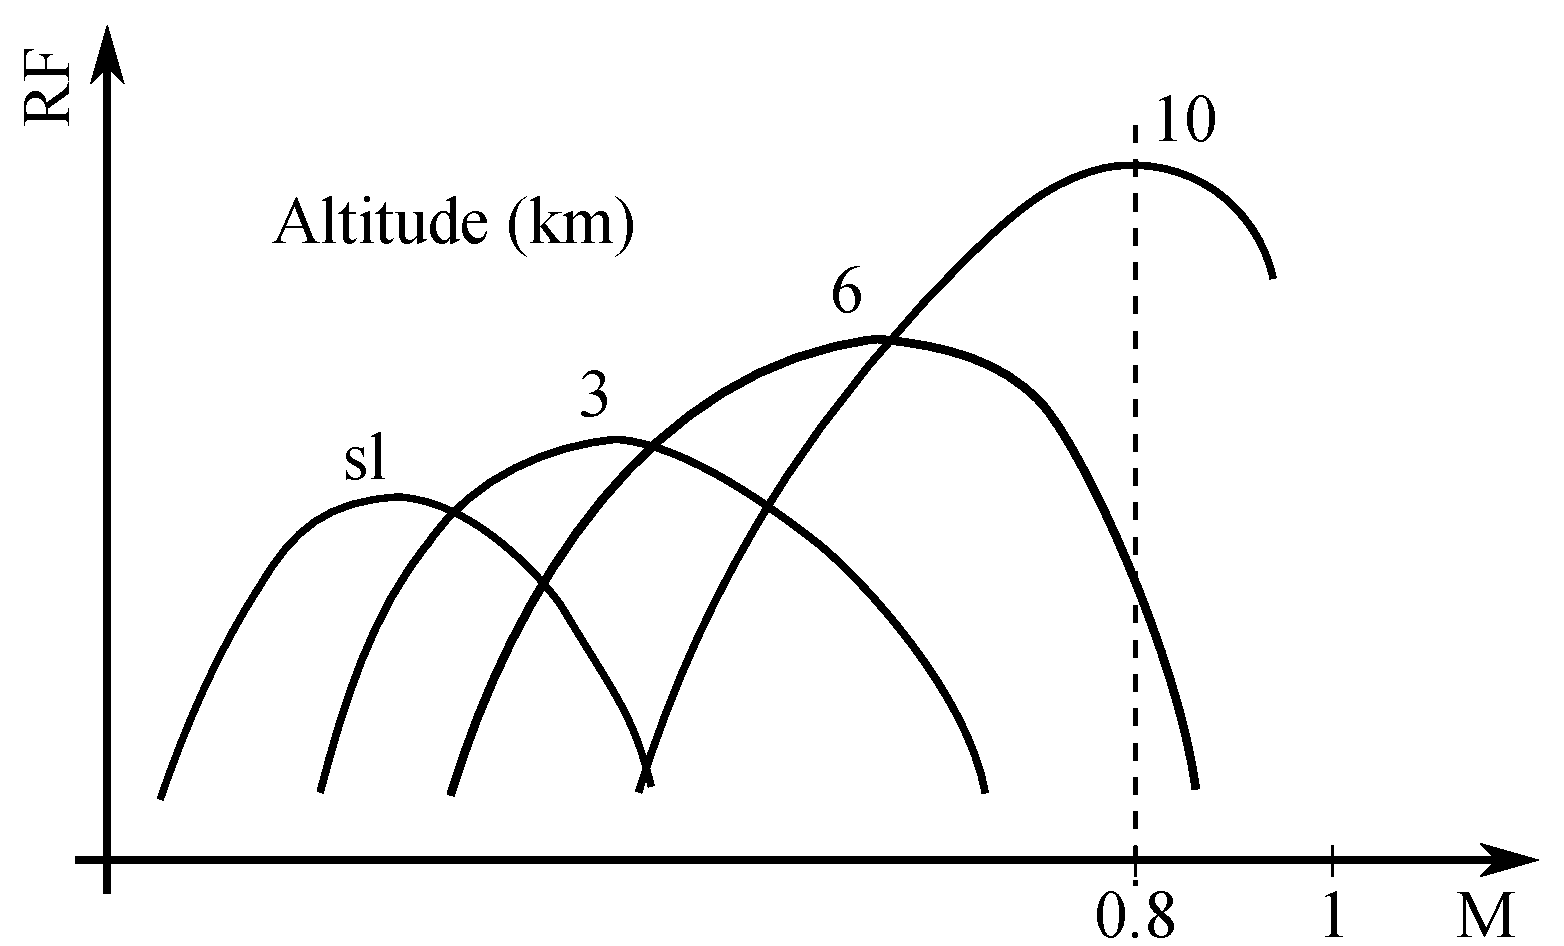
\includegraphics[width=0.48\textwidth]{RF}
    \caption{\label{fig:EFRF}Endurance factor and range factor.}
  \end{center}
\end{figure}
%================================================================

The TSFC is a function of engine, altitude and the flight Mach number. Some useful estimates for $\text{TSFC}_\text{I}$ (the subscript I means for $T_I$) are
\begin{itemizePacked}
\item High bypass-ratio turbofan engine:
  \begin{equation}
  \text{TSFC}_\text{I} = (0.4 + 0.45 \text{M}) \sqrt{\frac{T}{T_\text{ref}}} \, ;
  \end{equation}
\item LBR turbofan engine (military):
  \begin{equation}
  \text{TSFC}_\text{I} = (1.0 + 0.35 \text{M}) \sqrt{\frac{T}{T_\text{ref}}} \, ;
  \end{equation}
\item Turbojet (military):
  \begin{equation}
  \text{TSFC}_\text{I} = (1.3 + 0.26 \text{M}) \sqrt{\frac{T}{T_\text{ref}}} \, .
  \end{equation}
\end{itemizePacked}

%%%%%%%%%%%%%%%%%%%%%%%%%%%%%%%%%%%%%%%%%%%%%%%%%%%%%%%%%%%%%%%%%%
\subsection{Performance Parameters}
%%%%%%%%%%%%%%%%%%%%%%%%%%%%%%%%%%%%%%%%%%%%%%%%%%%%%%%%%%%%%%%%%%

%%%%%%%%%%%%%%%%%%%%%%%%%%%%%%%%%%%%%%%%%%%%%%%%%%%%%%%%%%%%%%%%%
\subsubsection{Thermal Efficiency}
%%%%%%%%%%%%%%%%%%%%%%%%%%%%%%%%%%%%%%%%%%%%%%%%%%%%%%%%%%%%%%%%%

%================================================================
\begin{figure}[!b!]
  \begin{center}
    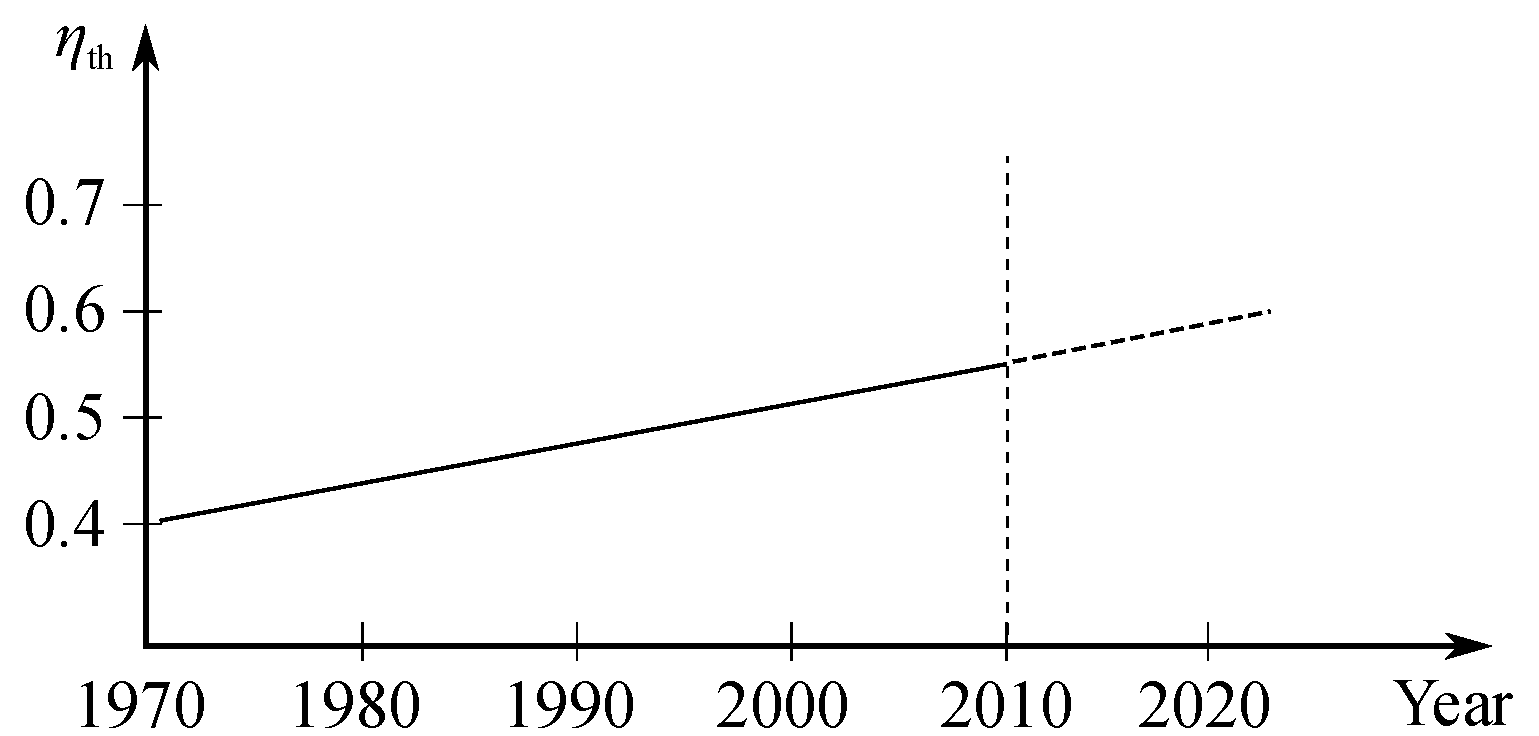
\includegraphics[width=0.58\textwidth]{etaThermal}
    \caption{\label{fig:ETA_THERMAL}Evolution of thermal efficiency over time.}
  \end{center}
\end{figure} 
%================================================================

The thermal efficiency is defined to be the net rate of power output (kinetic energy) over the available thermal energy:
\begin{equation}
  \eta_\text{th} = \f{\dot{P}_\text{out}}{\dot{Q}_\text{in}} = \f{\text{Net power of engine}}{\text{Heat addition by combustion}} \,,
\end{equation}
and
\begin{equation}
  \dot{P}_\text{out} = \f{1}{2} \dot{m}_F  \left[ \left( 1+\f{\dot{m}_A}{\dot{m}_F}\right)U_e^2-U_0^2\right]\,,
\end{equation}
which is the net rate of change of kinetic energy through the engine. The heat addition is defined as:
\begin{equation}
  \dot{Q}_\text{in} = \dot{m}_F \text{LHV}\,,
\end{equation}
where LHV is the lower heating value of fuel (which considers that the water that is formed in the combustion products remains in the vapor state). With this,
the thermal efficiency can be written as:
\begin{equation}
  \eta_\text{th} = \f{1}{2 \text{LHV}} \f{\dot{m}_A}{\dot{m}_F} \left[ \left( 1+\f{\dot{m}_A}{\dot{m}_F}\right)U_e^2-U_0^2\right]\,.
\end{equation}
\Cref{fig:ETA_THERMAL} shows the thermal efficiency as a function of year.

%%%%%%%%%%%%%%%%%%%%%%%%%%%%%%%%%%%%%%%%%%%%%%%%%%%%%%%%%%%%%%%%%
\subsubsection{Propulsive Efficiency}
%%%%%%%%%%%%%%%%%%%%%%%%%%%%%%%%%%%%%%%%%%%%%%%%%%%%%%%%%%%%%%%%%
The propulsive efficiency is a measure for how efficiently the engine power is used to power the aircraft:
\begin{equation}
  \label{EQ_ETA_P}
  \eta_p = \f{\text{Propulsive power of aircraft}}{\text{Net power of engine}} = \f{\dot{P}_p}{\dot{P}_\text{out}}\,,
\end{equation}
where $P_p = T_I U_0$ (with $T_I$ being the installed thrust) is the propulsive power. With this, the propulsive efficiency can be written as:
\begin{equation}
  \begin{split}
    \eta_p &= \f{T_IU_0}{\f{1}{2}\dot{m}_A\left[ \left( 1+\f{\dot{m}_A}{\dot{m}_F}\right)U_e^2-U_0^2\right]}\;,\\
               &= \f{(1-\phi_\text{inlet}-\phi_\text{nozzle})U_0\left\{\dot{m}_A\left[ \left( 1+\f{\dot{m}_A}{\dot{m}_F}\right)U_e^2-U_0^2\right] + A_C (p_e-p_0) \right\}}{\f{1}{2}\dot{m}_A\left[ \left( 1+\f{\dot{m}_A}{\dot{m}_F}\right)U_e^2-U_0^2\right]}\,.
  \end{split}
\end{equation}
For the case of (i) a perfectly expanded nozzle, (ii) $\dot{m}_F/\dot{m}_A=f \rightarrow 0$, and (iii) $T_I \rightarrow T_U$ with $\phi_\text{inlet} = 0$ and $\phi_\text{nozzle} = 0$, \cref{EQ_ETA_P} reduces to:
\begin{equation}
\label{eqn:etaPropulsive}
  \eta_p = \f{2U_0}{U_e+U_0} = \f{2}{1+\f{U_e}{U_0}}\,.
\end{equation}
\Cref{fig:ETA_PROPULSIVE} shows the propulsive as a function of $U_e / U_0$. From this figure it can be seen that we require $U_e\to U_0$ to achieve a maximum propulsive efficiency of unity. However, at this condition, no thrust is generated. Conditions with $U_e/U_0<1$ correspond to a wind generator in which we extract work from the air to generate power, and a windmill is a typical example for this.

%================================================================
\begin{figure}[!htb!]
  \begin{center}
    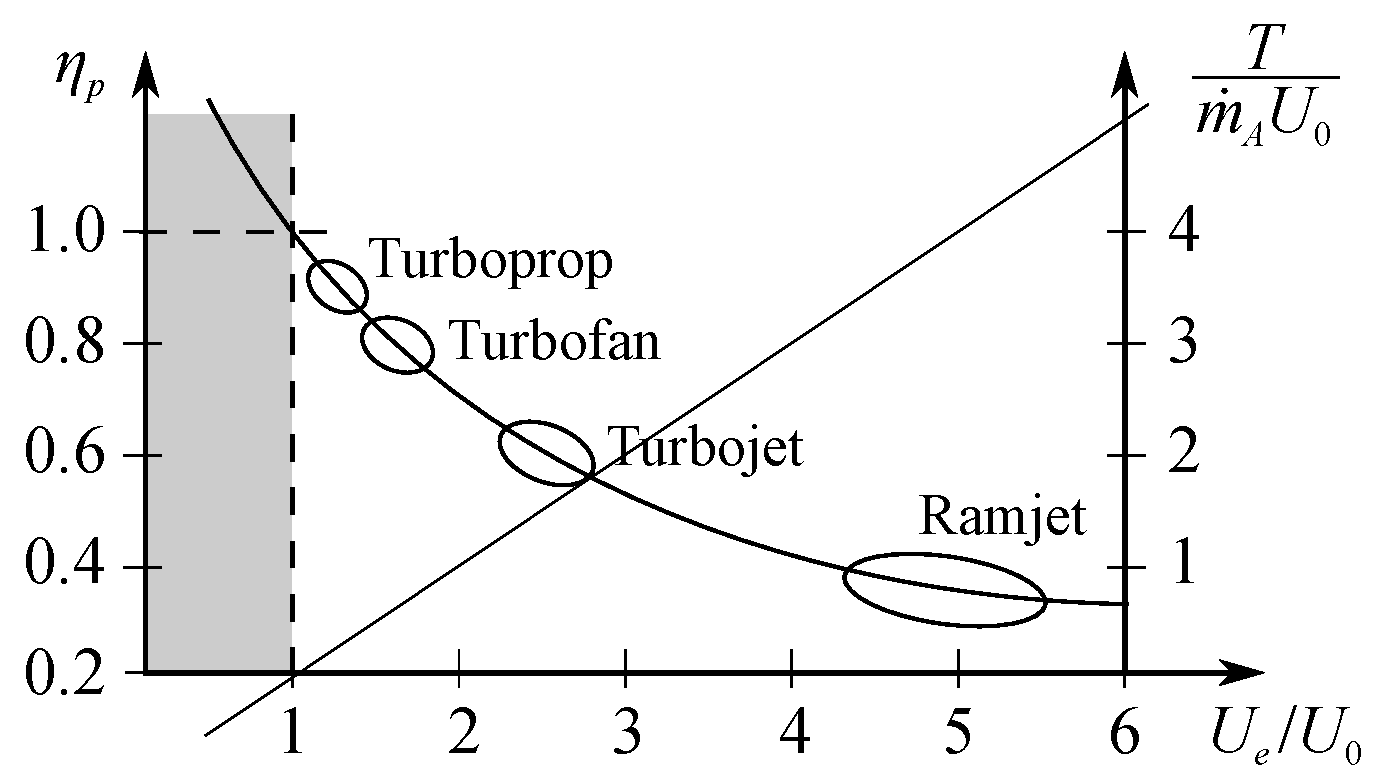
\includegraphics[width=0.56\textwidth]{etaPropulsive}
    \caption{\label{fig:ETA_PROPULSIVE}Propulsive efficiency.}
  \end{center}
\end{figure}
%================================================================

%%%%%%%%%%%%%%%%%%%%%%%%%%%%%%%%%%%%%%%%%%%%%%%%%%%%%%%%%%%%%%%%%
\subsubsection{Overall Efficiency}
%%%%%%%%%%%%%%%%%%%%%%%%%%%%%%%%%%%%%%%%%%%%%%%%%%%%%%%%%%%%%%%%%
The overall efficiency is defined as:
\begin{equation}
\begin{split}
  \eta_o &= \f{\text{Propulsive power}}{\text{Thermal power}}\\
             &= \eta_\text{th} \eta_p\\
             &= \f{\dot{P}_p}{\dot{Q}_\text{in}} = \f{T_I U_0}{\dot{Q}_\text{in}} = \f{T_I U_0}{\dot{m}_F \text{LHV}}\,.
\end{split}
\end{equation}
By introducing the definition for the installed thrust-specific fuel consumption $\text{TSFC}_\text{I} = \dot{m}_F/{T_I}$, this can be write as:
\begin{equation}
  \eta_o = \f{U_0}{\text{TSFC}_\text{I}\, \text{LHV}}\,.
\end{equation}
\Cref{fig:ETA_OVERALL} shows the overall efficiency as a function of both $\eta_\text{th}$ and $\eta_p$.

%================================================================
\begin{figure}[!htb!]
  \begin{center}
    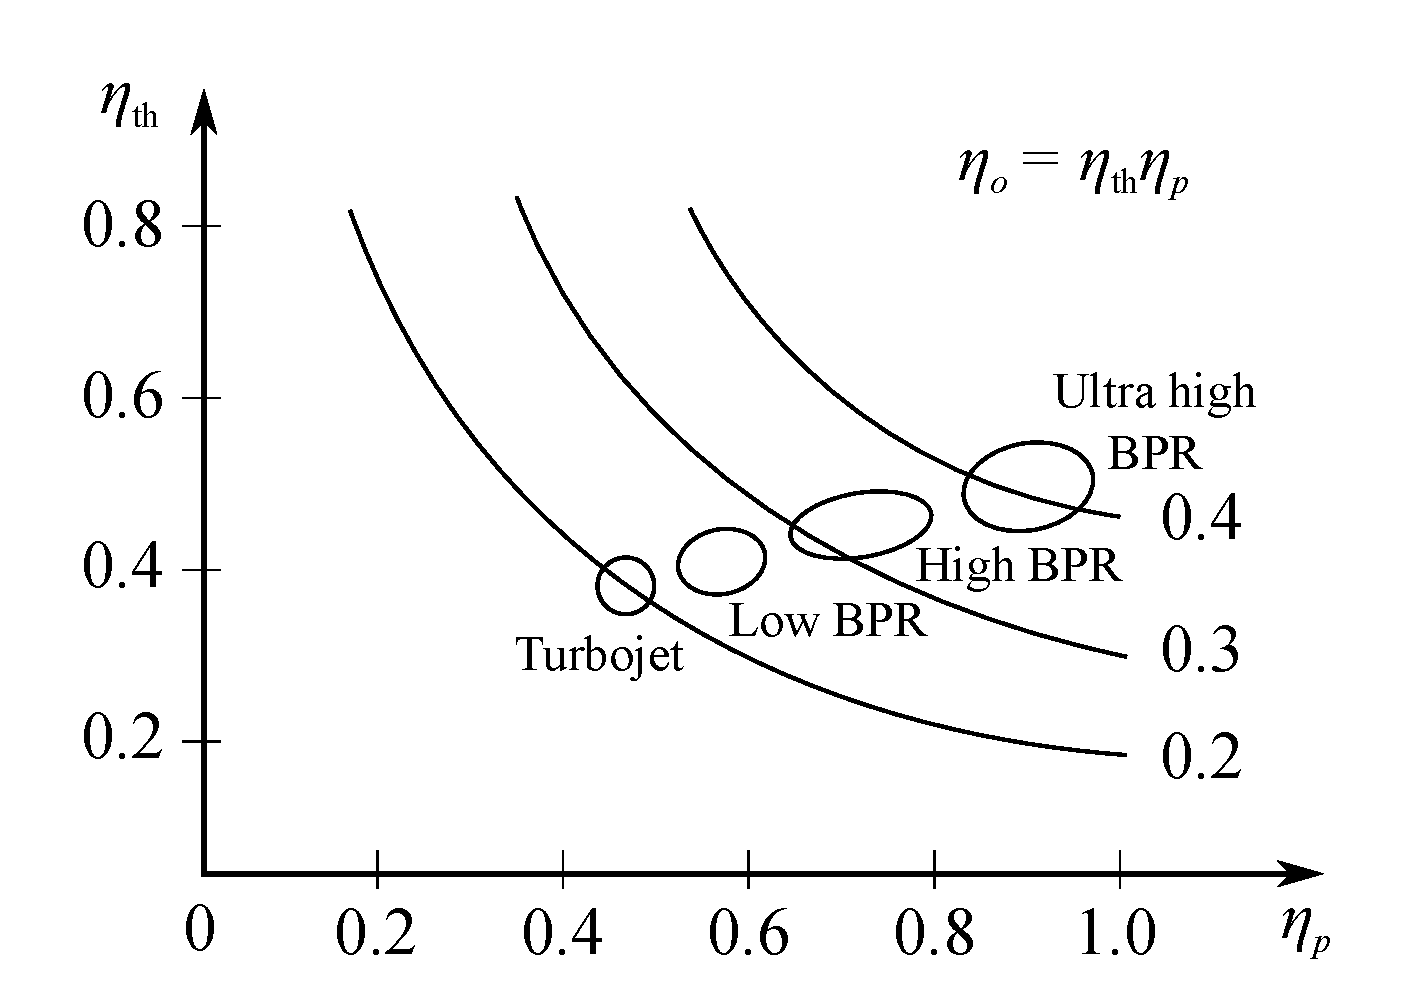
\includegraphics[width=0.54\textwidth]{etaThEtaP}
    \caption{\label{fig:ETA_OVERALL}Overall efficiency.}
  \end{center}
\end{figure}
%================================================================

%%%%%%%%%%%%%%%%%%%%%%%%%%%%%%%%%%%%%%%%%%%%%%%%%%%%%%%%%%%%%%%%%%
%\paragraph{Propeller Thrust}\mbox{} \\[0.5em]
%%%%%%%%%%%%%%%%%%%%%%%%%%%%%%%%%%%%%%%%%%%%%%%%%%%%%%%%%%%%%%%%%%
%Thrust generation by propeller is facilitated by imparting work to accelerate the fluid that passes through the propeller. Analysis of propeller performance follows classical turbomachinery analysis (see Sec. 7 of \cite{HILL_PETERSON_BOOK1992}; we will get back to this subject in our turbomachinery analysis to study compressor and turbine performance).
%
%To relate the propeller torque to the momentum difference across the propeller, we can conduct a kinematic analysis of the velocity field around a single propeller at a blade radius $r_B$. This analysis results in the so-called velocity-triangle. In this analysis, we differentiate between absolute (fixed coordinate systems) and relative (to blade) velocity:
%\begin{tabbing}
%  \qquad\= $U_\infty$: \= Fluid velocity, approach speed in fixed (absolute) coordinate systems;\\
%  \> $V_B$: \> Blade velocity, with $V_B = \Omega r_B$;\\
%  \> $W$: \> Fluid velocity, relative to rotating blade;\\
%  \> $\alpha$: \> absolute angle of attack;\\
%  \> $\beta$: \> blade angle.
%\end{tabbing}
%From the kinematic relation at the leading or trailing edge of the blade we can then construct the velocity triangle:
%\begin{equation}
% W + V_B = U_\infty \,.
%\end{equation}
%
%%================================================================
%\begin{figure}[!h!]
%  \begin{center}
%    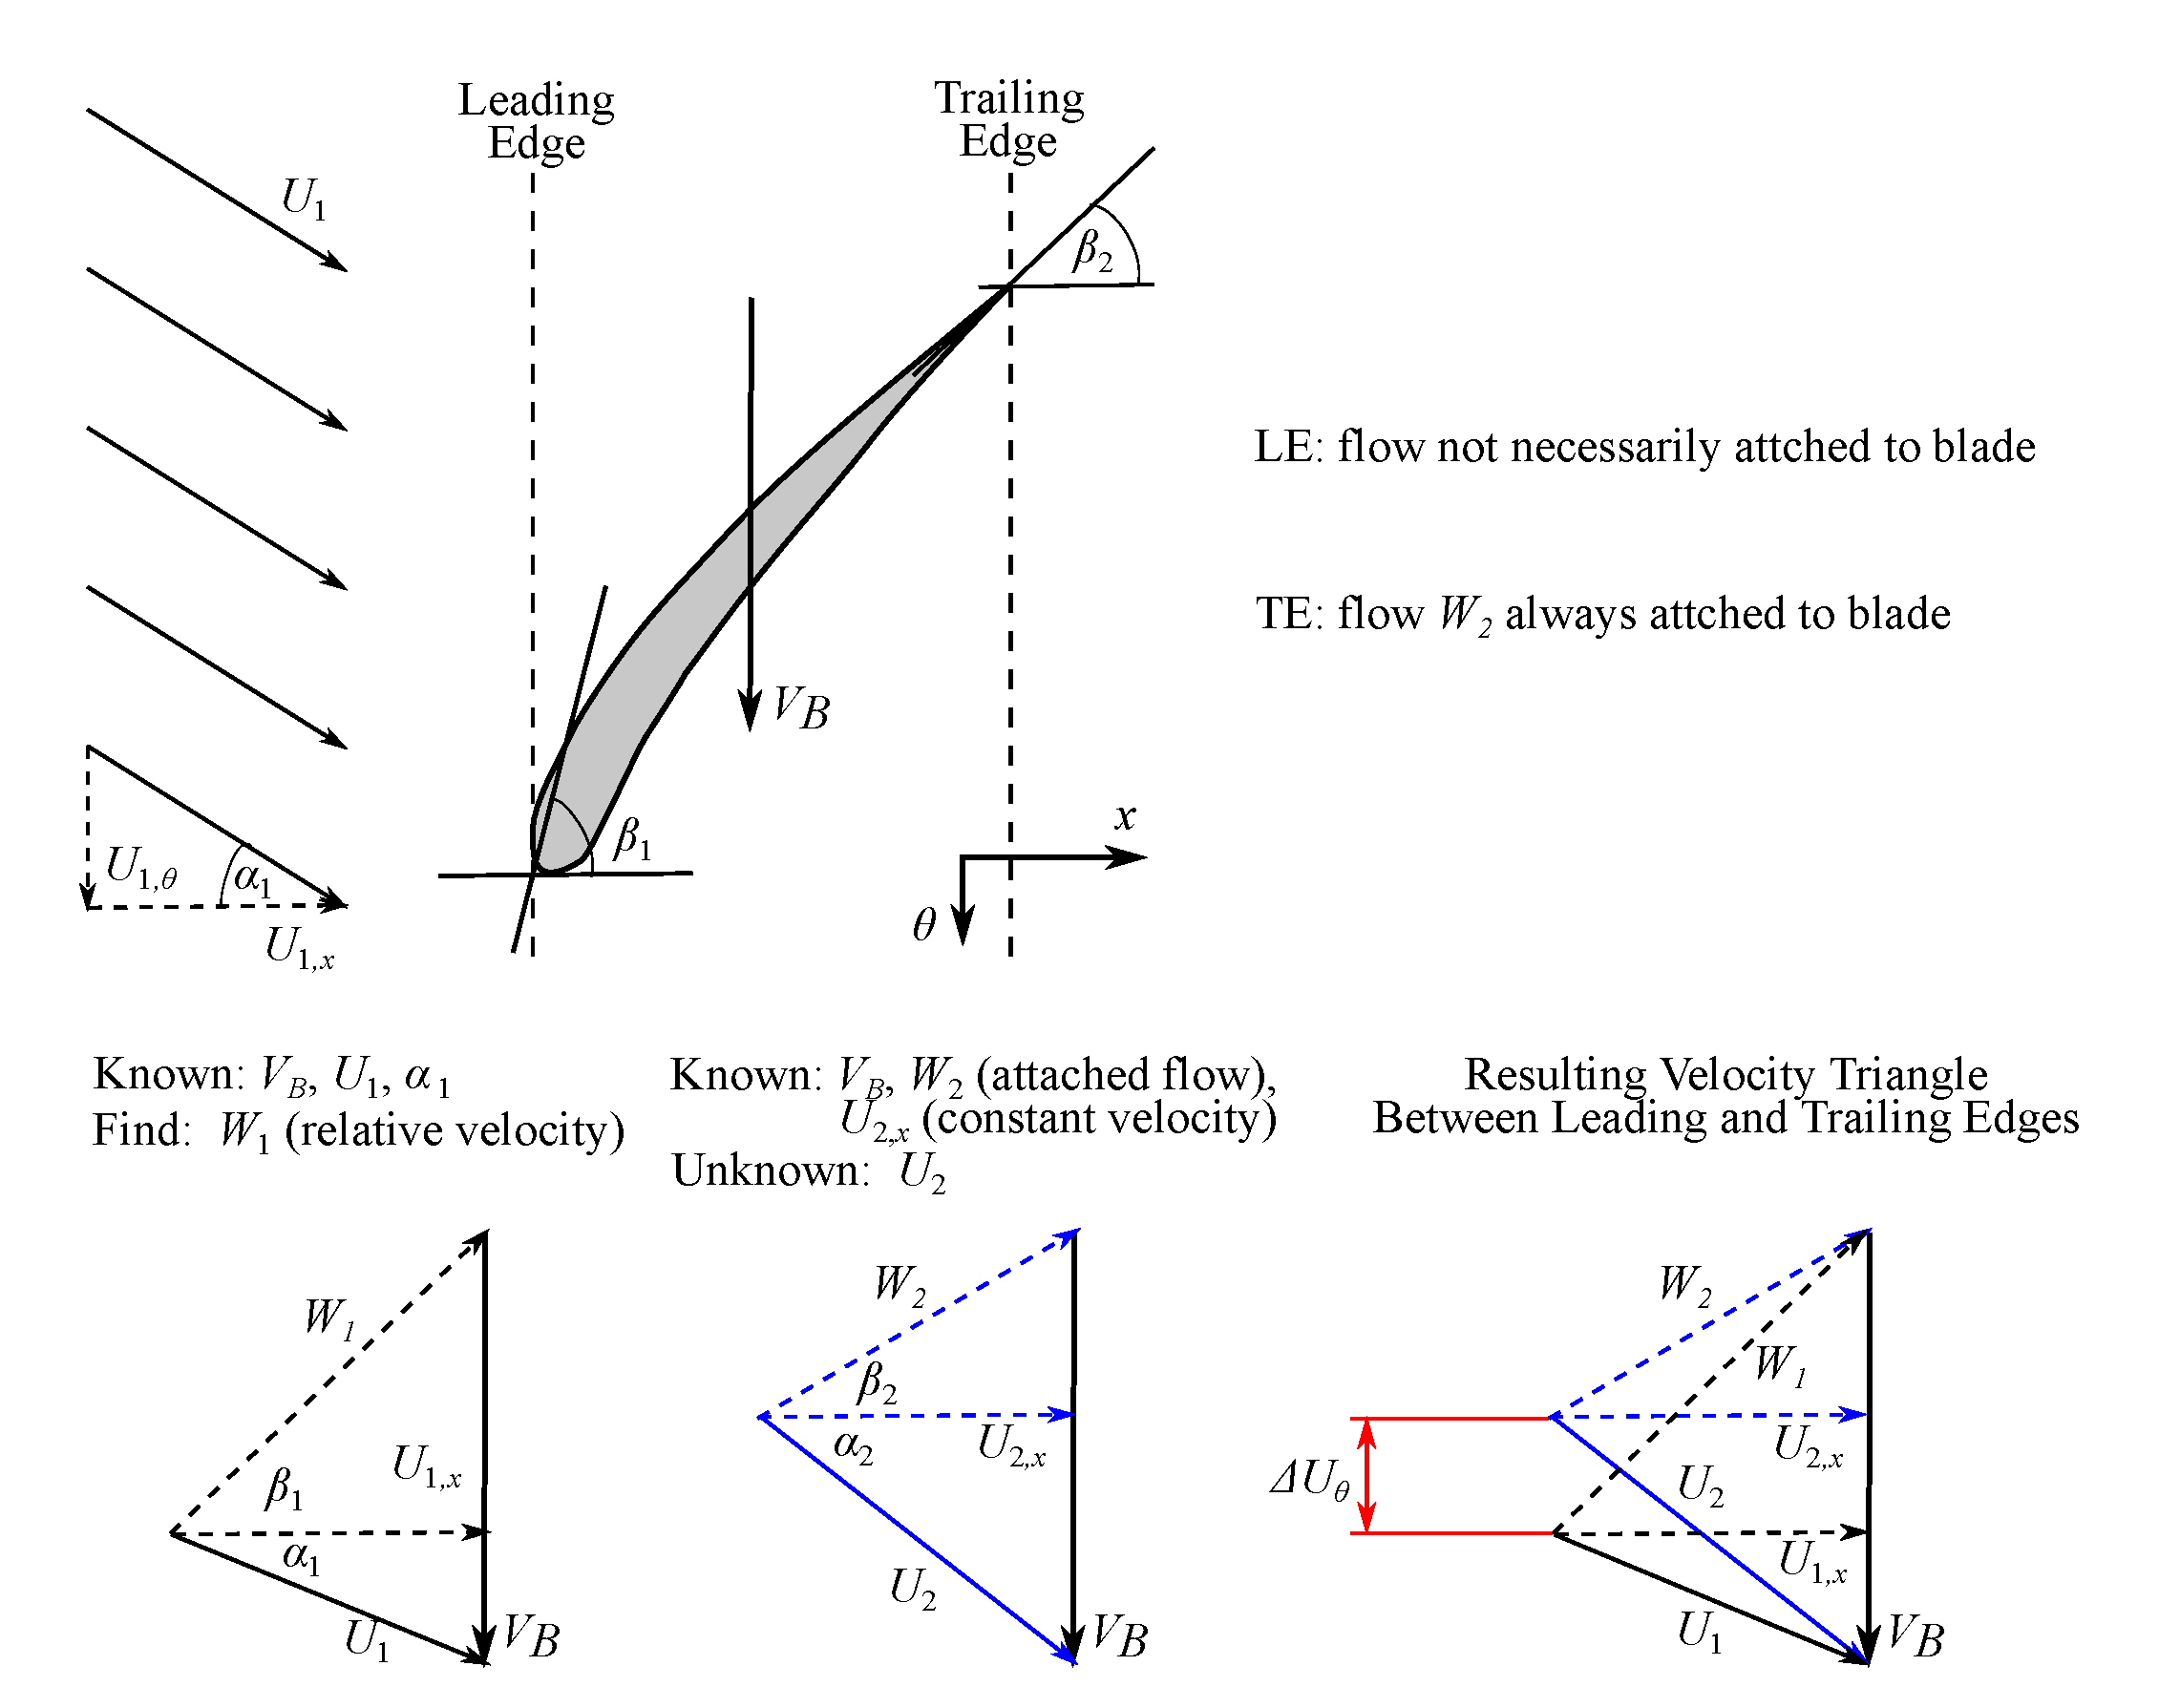
\includegraphics[width=0.95\textwidth]{velocityTriangle}
%  \caption{\label{FIG_VELOCITY_TRIANGLE}Velocity triangle.}
%  \end{center}
%\end{figure}
%%================================================================
%
%The construction of the velocity triangle at the leading and trailing edges of the propeller blade is illustrated in \cref{FIG_VELOCITY_TRIANGLE}. By superimposing both triangles, we can determine differences in azimuthal velocity components between trailing and leading edges:
%\begin{equation}
%  \Delta U_\theta = U_{\theta,2} - U_{\theta,1} \, \text{.}
%\end{equation}
%Similarly, we can also compute the axial velocity difference
%\begin{equation}
%  \Delta U_z = U_{z,2} - U_{z,1} \, \text{.}
%\end{equation}
%With this, we can evaluate the {\it torque} required to drive the propeller:
%\begin{equation}
%  \cT_{Prop}(r_B) = \dot{m}r_B\Delta U_{\theta} \, \text{,}
%\end{equation}
%or by considering a control area, we can evaluate the entire torque of the propeller
%\begin{equation}
%  \cT_{Prop} = N_{B} \int^R_0 2\pi \rho U_{\infty,z}r^2(\Delta U_\theta)dr \, \text{,}
%\end{equation}
%where $N_B$ is the number of blades.
%
%The propeller power is then evaluated as:
%\begin{equation}
%  \cP_{Prop} = \cT_{Prop}\Omega \, \text{,}
%\end{equation}
%where  $\Omega$ is the angular speed of the propeller (in units of s$^{-1}$). By accounting for the efficiency of the propeller in converting mechanical into technical work, we introduce a propeller efficiency $\eta_{Prop}$:
%\begin{equation}
%  \cP_{Prop} = {\eta_{Prop}}\cP_{Engine} \, \text{,}
%\end{equation}
%where $\cP_{Engine}$ is the required engine power. 
%
%With the thrust equation (derived in the next section) we can relate the axial velocity difference across the propeller to the thrust:
%\begin{equation}
% T = \dot{m}\Delta U_z \, \text{.}
%\end{equation}
%Note that we can typically neglect any area contraction or ram-effects upstream of the propeller, so that $U_\infty$ remains constant.
%
%%%%%%%%%%%%%%%%%%%%%%%%%%%%%%%%%%%%%%%%%%%%%%%%%%%%%%%%%%%%%%%%%%
%\paragraph{Propulsive Efficiency}\mbox{} \\[0.5em]
%%%%%%%%%%%%%%%%%%%%%%%%%%%%%%%%%%%%%%%%%%%%%%%%%%%%%%%%%%%%%%%%%%
%The {\it overall efficiency} is defined as:
%\begin{eqnarray}
%  \eta_O&=&\f{\text{Propulsive Power}}{\text{Total Power/Energy Available in Fuel}}\\
%        &=& \underbrace{\f{\text{Propulsive Power}}{\text{Flow Power}}}_{\text{Propulsive Efficiency $\eta_P$}}
%            \underbrace{\f{\text{Flow Power}}{\text{Total Power/Energy Available in Fuel}}}_{\text{Thermal Efficiency $\eta_{th}$}}
%\end{eqnarray}
%and with the definitions:
%\begin{tabbing}
%  \qquad\= Propulsive Power:\quad\= $P_P$\= $=TU_\infty$, \\
%  \> Flow Power: \> $P_F$\> $=KE_{out}-KE_{in}$\\[1mm]
%  \> \>\> $=\f{1}{2}\dot{m}_eU^2_e-\f{1}{2}\dot{m}_iU^2_\infty$\\[1mm]
%  \> \>\> $=\f{1}{2}\dot{m}_i\left[(1+f)U^2_e-U^2_\infty\right]$.
%\end{tabbing}
%
%The {\it propulsive efficiency} is defined as:
%\begin{eqnarray}
%  \eta_P&=&\f{TU_\infty}{\f{1}{2}\dot{m}_i[(1+f)U^2_e-U^2_\infty]} \, \text{,}
%\end{eqnarray}
%with \cref{EQ_THRUST_EQUATION} for the expression for thrust, and the thermal efficiency is specific to the thermodynamic cycle. After introducing the simplifications $f\ll1$ (with $f=\f{\dot{m}_f}{\dot{m}_{air}}$ being the fuel/air ratio) and pressure thrust $\ll$ jet thrust, we have
%\begin{equation}
%  \eta_P=\f{2}{\left(\f{U_e}{U_\infty}+1\right)}
%\end{equation}
%so that $0\le\eta_P\le2$. Maximizing $\eta_P$ requires $U_e\to 0.$ However, to maximize thrust we requires $U_e\to \infty$. \Cref{FIG_CV_ANALYSIS_THRUST_EQUATION} shows the variation of propulsive efficiency and thrust against velocity ratio.
%
%%================================================================
%\begin{figure}[t!]
%  \begin{center}
%    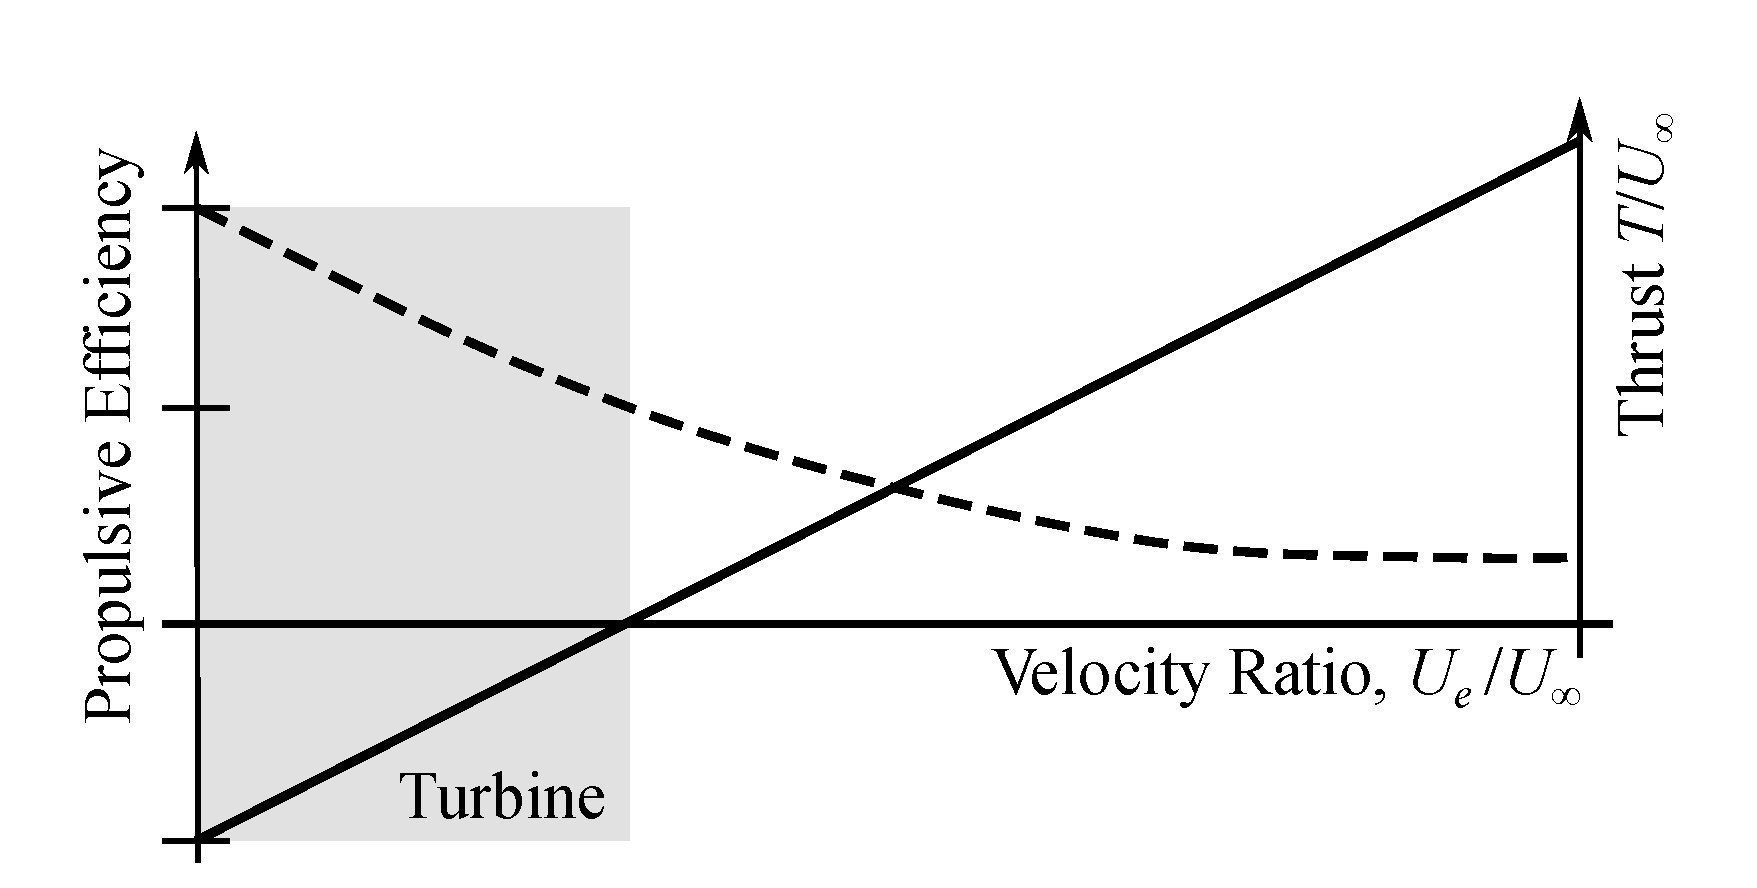
\includegraphics[width=0.6\textwidth]{efficiencyThrustCurve}
%    \caption{\label{FIG_CV_ANALYSIS_THRUST_EQUATION}Propulsive efficiency and thrust vs. velocity ratio.}
%  \end{center}
%\end{figure}
%%================================================================
%\vspace*{1in}

